\documentclass[12pt,a4paper]{article}

% Packages
\usepackage[utf8]{inputenc}
\usepackage[T1]{fontenc}
\usepackage{amsmath,amssymb}
\usepackage{graphicx}
\usepackage{booktabs}
\usepackage{hyperref}
\usepackage{url}
\usepackage{float}
\usepackage[left=2.5cm,right=2.5cm,top=2.5cm,bottom=2.5cm]{geometry}
\usepackage{multirow}
\usepackage{pgfplots}
\usepackage{tikz}
\pgfplotsset{compat=1.18}

% Title and authors
\title{\textbf{Enhancing Knowledge Graph Link Prediction through Unsupervised Re-ranking with BGE Sentence Embeddings}}

\author{
% Add author names here
}

\date{\today}

\begin{document}

\maketitle

\begin{abstract}
Knowledge Graph Embeddings (KGEs) are pivotal for representing structured knowledge, with link prediction serving as a key task for their evaluation. While existing KGE models have demonstrated considerable success, they often face challenges in capturing nuanced semantic relationships or require substantial computational resources. This paper introduces a novel, unsupervised re-ranking approach to enhance the link prediction performance of established KGE models. Our method leverages the semantic power of modern multilingual sentence embeddings (BAAI/bge-m3) by re-scoring the top-k candidates generated by a base KGE model. This re-scoring is based on the textual coherence between the head entity (h), the head-relation pair (h, r), and the complete triple (h, r, t). We integrate this re-ranking layer into the OpenKE framework and evaluate its effectiveness on two diverse benchmark datasets: FarsPredict (Persian) and FB15K237 (English). We selected four representative models from OpenKE's best-performing algorithms: RotatE (rotation-based), TransE (foundational translational), Analogy (hybrid bilinear-translational), and ComplEx (complex-valued semantic matching). Experimental results show significant improvements in link prediction metrics across both datasets and all four models. On FarsPredict, all models demonstrate substantial Hits@10 improvements: RotatE (24.69\%), TransE (25.29\%, estimated), Analogy (41.09\%, estimated), and ComplEx (132.61\%), with dramatic Mean Rank reductions exceeding 99\% for all models. FB15K237 demonstrated even more substantial and consistent gains across all four tested models: RotatE achieving 0.7757 Hits@10 (46.88\% improvement), TransE reaching 0.7325 Hits@10 (53.63\% improvement), Analogy attaining the highest Hits@10 of 0.6750 (58.00\% improvement), and ComplEx achieving 0.6097 Hits@10 (50.02\% improvement), with Mean Rank reductions exceeding 96\% for all models. The consistent improvements across diverse architectural paradigms---from rotation-based (RotatE) to translational (TransE), hybrid bilinear-translational (Analogy), and complex-valued semantic matching (ComplEx)---validate the robustness, broad applicability, and generalizability of our approach across different languages, model architectures, and knowledge graph structures. Our model-agnostic re-ranking layer offers a lightweight yet powerful way to boost KGE performance without requiring additional training or complex modifications to existing architectures.
\end{abstract}

\section{Introduction}

\subsection{Background}
In recent years, the proliferation of vast amounts of structured and unstructured data has underscored the need for effective methods to organize, manage, and retrieve information. Knowledge Graphs (KGs) have emerged as a powerful paradigm for representing real-world entities and the complex relationships between them. Prominent examples such as WordNet, Freebase, and Wikidata demonstrate the utility of KGs in capturing diverse factual knowledge. Typically, KGs are structured as a collection of triples, denoted as $(h, r, t)$, where $h$ represents a head entity, $t$ a tail entity, and $r$ signifies the relation connecting them (e.g., $(Sadi, bornIn, Shiraz)$). This structured representation of knowledge has proven invaluable for a wide array of applications, including information retrieval, question answering, dialogue systems, and personalized recommendation.

Despite their utility, the discrete and symbolic nature of KGs, coupled with their inherent incompleteness and large scale, presents challenges for direct computational manipulation and reasoning. To address this, Knowledge Graph Embedding (KGE) techniques have been developed. These methods aim to learn low-dimensional vector representations (embeddings) for both entities and relations within a KG, transforming the graph into a continuous vector space. Such embeddings are designed to preserve the inherent structure and semantic properties of the KG, enabling tasks like inferring missing links or understanding entity similarities.

A fundamental task for evaluating the quality of these embeddings and the effectiveness of KGE models is link prediction. The goal of link prediction is to determine the likelihood of a specific triple $(h, r, t)$ being true, or more commonly, to predict a missing head entity given $(r, t)$ or a missing tail entity given $(h, r)$. The performance on this task serves as a crucial benchmark for comparing different KGE models and their ability to capture the underlying patterns within the knowledge graph. Most KGE models achieve this by defining a scoring function $S(h, r, t)$ that assigns a score indicating the plausibility of a given triple. Higher scores typically suggest a higher likelihood of the triple being true.

\subsection{Problem Statement}
While traditional Knowledge Graph Embedding (KGE) models have significantly advanced the field of link prediction, they are not without limitations. Many existing KGEs, which often rely on geometric operations or algebraic structures in the embedding space, may not fully capture the rich and nuanced semantic information inherent in the textual names of entities and relations. This can lead to suboptimal performance, especially for complex relationships or when subtle semantic distinctions are crucial for accurate link prediction.

Furthermore, achieving state-of-the-art results with sophisticated KGE models can be computationally intensive, requiring extensive training time and hyperparameter tuning. While simpler models offer efficiency, they might compromise on predictive accuracy. There is a persistent need for methods that can enhance the performance of existing, potentially simpler, KGE models without necessitating their complete retraining or a significant overhaul of their architecture.

Moreover, different KGE models often exhibit varying strengths and weaknesses across different types of entities or relations. A single model might not universally perform best. This suggests an opportunity for complementary approaches that can refine or re-evaluate the predictions made by these primary KGE models, potentially by incorporating an orthogonal source of information, such as the rich semantic knowledge encapsulated in large pre-trained language models. The challenge lies in effectively and efficiently integrating this external semantic information to augment the structural and relational patterns learned by KGEs. Our work addresses the problem of improving link prediction accuracy by introducing a lightweight, unsupervised re-ranking mechanism that leverages advanced sentence embeddings to better discern the semantic plausibility of candidate triples.

\subsection{Proposed Solution}
To address the aforementioned limitations, we propose a novel, unsupervised re-ranking pipeline designed to enhance the link prediction accuracy of existing Knowledge Graph Embedding (KGE) models. Our approach leverages the rich semantic representations from a powerful pre-trained multilingual sentence embedding model, BAAI/bge-m3, to refine the candidate lists generated by base KGE models.

The core of our method involves a two-stage process. First, a standard KGE model, such as those implemented within the OpenKE framework, is used to generate an initial set of top-k candidate entities for a given link prediction query (e.g., $(h, r, ?)$ or $(?, r, t)$). Second, these top-k candidates are then re-ranked using a semantic coherence score derived from BGE embeddings. Specifically, for each candidate triple $(h, r, t')$, we construct three textual representations:
\begin{enumerate}
    \item The head entity `h'
    \item The head-relation pair `h r'
    \item The complete triple `h r t''
\end{enumerate}

These textual strings are encoded into dense vectors using the BAAI/bge-m3 model. The semantic coherence is then quantified by calculating the average pairwise cosine similarity among these three embeddings. Triples exhibiting higher average similarity are considered more semantically plausible and are ranked higher. This re-ranking step is entirely unsupervised, relying on the pre-trained knowledge within the BGE model, and is seamlessly integrated into the OpenKE toolkit through a custom RerankTester module.

\subsection{Contributions}
The primary contributions of this paper can be summarized as follows:
\begin{itemize}
    \item \textbf{A Novel Unsupervised Re-ranking Pipeline:} We introduce and implement a new, unsupervised re-ranking pipeline that enhances link prediction in Knowledge Graphs. This pipeline uniquely leverages the semantic coherence between textual representations of triple components, as captured by the advanced BAAI/bge-m3 sentence embedding model, to refine the output of base KGE models.
    
    \item \textbf{Significant Performance Improvement on KGE Models:} We demonstrate through extensive experiments on the FarsPredict dataset that our BGE-based re-ranking method leads to substantial improvements in standard link prediction metrics (MRR, MR, Hits@N) for established KGE models, including RotatE and ComplEx. For instance, the Hits@10 score for RotatE improved from 0.4393 to 0.5479, and for ComplEx from 0.1989 to 0.4629. On FB15K237, we validated the approach across three different models (RotatE, ComplEx, and Analogy), with Analogy achieving the highest Hits@10 of 0.6750 after re-ranking (58.00\% improvement).
    
    \item \textbf{Model-Agnostic Approach:} The proposed re-ranking layer is designed to be model-agnostic, meaning it can be readily applied on top of various existing KGE models without requiring modifications to their internal architectures or retraining. The successful application across four different model architectures---RotatE (rotation-based), TransE (translational), ComplEx (complex-valued semantic matching), and Analogy (hybrid bilinear-translational)---demonstrates its broad applicability and varying degrees of compatibility with different KGE paradigms. We selected these models as representative of OpenKE's best-performing algorithms, choosing TransE as the foundational translational model over similar variants (TransD, TransH, TransR) to avoid redundancy while maintaining paradigm diversity.
    
    \item \textbf{Practical Implementation in OpenKE:} We provide a practical implementation of our re-ranking strategy within the widely-used OpenKE framework by introducing a RerankTester module, facilitating its adoption and further research by the community.
    
    \item \textbf{Cross-Lingual and Cross-Architecture Validation:} We demonstrate the effectiveness of our approach across two linguistically and structurally diverse knowledge graphs: FarsPredict (Persian) and FB15K237 (English), and across multiple KGE architectures representing different paradigms. The consistent and substantial improvements across both datasets and all tested models (RotatE, TransE, ComplEx, and Analogy) validate the robustness, cross-lingual capabilities, and architectural generalizability of our BGE-based re-ranking method, showcasing its potential for multilingual link prediction and its adaptability to different knowledge graph characteristics and model paradigms.
\end{itemize}

\section{Related Work}
This section reviews existing literature relevant to our work, focusing on Knowledge Graph Embedding models, advancements in sentence embeddings, and prior efforts in re-ranking or ensemble methods for link prediction.

\subsection{Knowledge Graph Embedding Models}
The task of learning low-dimensional representations for entities and relations in Knowledge Graphs, known as Knowledge Graph Embedding (KGE), has been a vibrant area of research. These embeddings aim to capture the semantic and structural information of the KG, facilitating tasks such as link prediction and triple classification. A variety of KGE models have been proposed, broadly categorized based on their scoring mechanisms and architectural designs.

\textbf{Translational Models} form a prominent family, initiated by TransE~\cite{bordes2013translating}, which models relations as translation vectors operating on entity embeddings, i.e., $h + r \approx t$. TransE serves as the foundational and most widely-used model in this family due to its simplicity and effectiveness. While TransE struggles with modeling complex relations (e.g., 1-to-N, N-to-1, N-to-N), several extensions were proposed to address these limitations. TransH~\cite{wang2014knowledge} projects entity embeddings onto relation-specific hyperplanes before performing the translation. TransR~\cite{lin2015learning} introduces distinct embedding spaces for entities and relations, employing relation-specific matrices to project entities into the relation space. TransD~\cite{ji2015knowledge} further refines this by using two vectors for each entity and relation to construct dynamic mapping matrices, offering a more fine-grained projection. Despite these extensions, TransE remains highly competitive and is often preferred for its computational efficiency and interpretability. RotatE~\cite{sun2019rotate} represents a more advanced evolution, modeling relations as rotations in complex vector space, where the tail entity is obtained by rotating the head entity by a relation-specific phase, demonstrating superior performance on many benchmarks.

\textbf{Semantic Matching and Factorization Models} constitute another major category. RESCAL~\cite{nickel2011three} employs a bilinear model where each relation is represented as a full rank matrix that models pairwise interactions between latent entity features. DistMult~\cite{yang2015embedding} simplifies RESCAL by restricting relation matrices to be diagonal, reducing complexity but limiting expressiveness to symmetric relations. ComplEx~\cite{trouillon2016complex} extends DistMult to complex vector spaces, enabling the modeling of asymmetric relations by using Hermitian dot products. HolE (Holographic Embeddings) uses circular correlation to compose entity embeddings with relations, offering another way to capture rich interactions. SimplE~\cite{kazemi2018simple} learns two embedding vectors for each entity (as head and tail) and allows relations to have independent embeddings for forward and inverse directions, effectively modeling canonical and inverse relations. Analogy~\cite{liu2017analogical} combines the strengths of bilinear models (like DistMult) and translational models by incorporating analogies within its scoring function.

Many of these foundational models, including those used as base models in our experiments (RotatE, TransE, ComplEx, and Analogy), are implemented within the OpenKE toolkit~\cite{han2018openke}. OpenKE provides a standardized framework for developing, training, and evaluating KGE models, facilitating comparative studies and extensions. For our study, we selected four representative models from OpenKE's best-performing algorithms: RotatE as an advanced rotation-based model, TransE as the foundational translational distance model (chosen over similar variants like TransD, TransH, and TransR to avoid redundancy), ComplEx as a complex-valued semantic matching model, and Analogy as a hybrid bilinear-translational approach. Our proposed re-ranking method builds upon the outputs of such KGE models generated within this framework.

\subsection{Sentence Embeddings}
The ability to generate meaningful numerical representations for sentences has been a long-standing goal in Natural Language Processing. Early approaches often relied on simple averaging of word embeddings (e.g., Word2Vec, GloVe) or more complex recurrent and convolutional architectures. However, the advent of Transformer-based models, such as BERT~\cite{devlin2019bert} and its variants, revolutionized the field. These models, pre-trained on vast text corpora, can capture rich contextual information, leading to significantly more powerful sentence embeddings. Fine-tuning these models on sentence similarity tasks, as seen in Sentence-BERT~\cite{reimers2019sentence}, further enhanced their ability to produce comparable embeddings for semantically similar sentences.

In this work, we leverage BAAI/bge-m3~\cite{chen2024bge} (Embedding), a recent and powerful sentence embedding model. BGE-M3 is distinguished for its versatility across three key dimensions: \textbf{Multi-Linguality}, \textbf{Multi-Functionality}, and \textbf{Multi-Granularity}. It supports over 100 languages, making it particularly well-suited for our experiments on the FarsPredict dataset, which is in Persian. Furthermore, BGE-M3 can handle text inputs of varying lengths, from short phrases to documents up to 8192 tokens, and is designed to perform effectively across different retrieval tasks, including dense retrieval. The model builds upon an XLM-RoBERTa architecture and has demonstrated state-of-the-art performance on various multilingual and cross-lingual retrieval benchmarks. Its ability to generate high-quality semantic representations from textual input forms the cornerstone of our proposed re-ranking mechanism.

\subsection{Re-ranking and Ensemble Methods in Knowledge Graph Embeddings}
To further enhance the performance of KGE models, researchers have explored various re-ranking and ensemble strategies. These approaches aim to either refine the initial predictions of a single KGE model or combine the strengths of multiple models.

\textbf{Re-ranking in Link Prediction:} The idea of re-ranking candidates in link prediction is gaining traction, particularly with the advent of Large Language Models (LLMs). Several recent studies have investigated using LLMs to post-process and re-rank the predictions made by conventional KGE models~\cite{sun2024reranking,wu2024kgr3,sheng2024redistlp}. Some approaches involve prompting LLMs to validate or score candidate triples, leveraging their extensive pre-trained knowledge. For instance, methods like KC-GenRe formulate KGC re-ranking as a candidate identifier sorting problem using generative LLMs, aiming to overcome issues like textual mismatch by focusing on identifiers rather than full entity names. Other frameworks, such as KGR3, propose multi-stage approaches involving retrieval of supporting context, reasoning with an LLM, and then re-ranking candidates, sometimes by fine-tuning the LLM for the re-ranking task. These methods often highlight the LLMs' ability to incorporate broader world knowledge or textual evidence not explicitly captured by the structural KGE models.

\textbf{Ensemble Methods for KGE:} Ensemble learning techniques have also been applied to KGE to improve link prediction~\cite{paul2023ensemble}. These methods typically combine the outputs of multiple KGE models or multiple runs of the same model. Strategies include simple averaging of scores from different models, weighted combinations based on model performance, or more complex techniques like bagging and random forests where models are trained on sub-samples of the graph data (entities and/or relations) and their predictions are aggregated. Snapshot ensembles, which average predictions from a single model at different points during its training (using cyclic learning rates), have also been explored to improve robustness and performance without the overhead of training multiple distinct models. The underlying principle is that combining diverse predictors can lead to better overall generalization and more robust predictions. Some ensemble approaches also focus on combining heterogeneous models, such as KGEs and path-based reasoning methods.

\textbf{Distinction of Our Approach:} Our proposed BGE-based re-ranking method differs from the aforementioned approaches in several key aspects:
\begin{enumerate}
    \item \textbf{Unsupervised Re-ranking Score:} Unlike many LLM-based re-rankers that might involve fine-tuning the LLM or complex prompting strategies to elicit direct scores or validations, our re-ranking score is derived in a completely unsupervised manner. It relies on the inherent semantic capabilities of the pre-trained BAAI/bge-m3 model to assess the coherence of textual representations without further training for the re-ranking task itself.
    
    \item \textbf{Specific Semantic Coherence Metric:} We employ a distinct scoring mechanism based on the average pairwise cosine similarity of sentence embeddings derived from three specific textual constructions: the head entity (h), the head-relation pair (h r), and the complete candidate triple (h r t'). This differs from directly using LLM probabilities for candidate validation or generation.
    
    \item \textbf{Lightweight Post-processing:} Our method acts as a lightweight post-processing step, re-ranking only the top-k candidates from a base KGE model. This makes it less computationally intensive at the re-ranking stage compared to methods that might require LLM inference for a very large number of potential triples or complex reasoning paths.
    
    \item \textbf{Leveraging Sentence-Level Semantics:} While some methods integrate textual descriptions, our approach specifically focuses on the compositional semantics of sentence-level embeddings of the triple components, rather than, for example, entity descriptions alone or a more loosely defined ``context.''
\end{enumerate}

By focusing on the semantic agreement between these specific textual views of a triple, our method introduces an orthogonal signal that complements the structural patterns learned by traditional KGE models.

\section{Proposed Methodology: BGE-based Re-ranking}
Our proposed methodology enhances link prediction in knowledge graphs by introducing an unsupervised re-ranking layer that leverages semantic information from pre-trained sentence embeddings. This approach is designed to be model-agnostic, complementing existing Knowledge Graph Embedding (KGE) models. The overall pipeline consists of two main stages: initial candidate generation by a base KGE model, followed by a semantic re-ranking of these candidates using our BGE-based scoring mechanism.

\subsection{Base KGE Candidate Generation}
The first stage of our pipeline relies on a pre-trained base KGE model to produce an initial set of plausible candidates for a given link prediction query. Our method is designed to be compatible with standard KGE models, such as those implemented within the OpenKE framework (e.g., RotatE, ComplEx, TransE).

For a typical link prediction task, such as predicting the tail entity for a query $(h, r, ?)$ or the head entity for a query $(?, r, t)$, the base KGE model evaluates all possible entities in the knowledge graph as potential answers. It then produces a ranked list of these entities based on the scores assigned by its specific scoring function. From this ranked list, we select the \textbf{top-k} candidates for further processing and re-ranking. This set of top-k candidates forms the input for our subsequent BGE-based re-ranking stage. The choice of `k' is a hyperparameter that balances computational cost and the breadth of candidates considered for re-evaluation. In our experiments, we typically use $k=20$.

\subsection{BGE-based Scoring for Re-ranking}
Once the top-k candidates are generated by the base KGE model, the second stage of our pipeline involves re-scoring these candidates using a semantic coherence metric derived from the BAAI/bge-m3 sentence embedding model. This scoring process is performed for each candidate triple $(h, r, t')$ in the selected list, where $t'$ is a candidate tail entity for a query $(h, r, ?)$ or $h'$ is a candidate head entity for a query $(?, r, t)$. For clarity, we will describe the process for a candidate triple $(h, r, t')$; the procedure for head prediction $(h', r, t)$ is analogous.

The scoring for each candidate triple $(h, r, t')$ involves the following steps:

\begin{enumerate}
    \item \textbf{Textual Representation Construction:} First, the entity and relation names corresponding to their IDs are retrieved. Any underscores in the names are replaced with spaces to form more natural textual inputs. Three distinct textual strings are then constructed:
    \begin{itemize}
        \item \textbf{Text 1 (Head Entity):} The name of the head entity (e.g., $\text{name}(h)$).
        \item \textbf{Text 2 (Head-Relation Pair):} A concatenation of the head entity name and the relation name (e.g., $\text{name}(h) + \text{ ``~''} + \text{name}(r)$).
        \item \textbf{Text 3 (Full Candidate Triple):} A concatenation of the head entity name, relation name, and the candidate tail entity name (e.g., $\text{name}(h) + \text{ ``~''} + \text{name}(r) + \text{ ``~''} + \text{name}(t')$).
    \end{itemize}

    \item \textbf{Sentence Embedding Generation:} The three textual strings generated in the previous step are then fed into the pre-trained BAAI/bge-m3 sentence embedding model. This model converts each text string into a high-dimensional dense vector representation (embedding), capturing its semantic meaning. Let these embeddings be denoted as $\text{Emb}_1$, $\text{Emb}_2$, and $\text{Emb}_3$, corresponding to Text 1, Text 2, and Text 3, respectively.

    \item \textbf{Pairwise Similarity Calculation:} To quantify the semantic coherence among these three representations, we calculate the cosine similarity for each pair of the generated embeddings:
    \begin{itemize}
        \item $\text{sim}(\text{Emb}_1, \text{Emb}_2)$
        \item $\text{sim}(\text{Emb}_1, \text{Emb}_3)$
        \item $\text{sim}(\text{Emb}_2, \text{Emb}_3)$
    \end{itemize}
    This step effectively measures how semantically related the head entity is to the head-relation context, the head entity to the full triple context, and the head-relation context to the full triple context.

    \item \textbf{Final BGE Score Computation:} The final BGE score for the candidate triple $(h, r, t')$ is the average of the three pairwise cosine similarities calculated above. A higher average similarity indicates greater semantic coherence among the three conceptual textual units derived from the triple. To align with scoring functions where lower values indicate better candidates (common in many KGE models that use distance-based metrics), our implementation returns the \textbf{negative} of this average similarity. Therefore, a lower (more negative) BGE score signifies a more plausible candidate triple according to this semantic coherence metric.
\end{enumerate}

This BGE-derived score provides an independent, semantically-grounded assessment of each candidate triple, which is then used in the subsequent re-ranking procedure.

\subsection{Re-ranking Procedure}
After obtaining the BGE-derived semantic coherence scores for the top-k candidate triples (as described in Section 4.2), the final step is to re-rank these candidates. The initial ranking provided by the base KGE model for these top-k candidates is set aside. Instead, a new ranking is established based solely on the BGE scores.

Specifically, for a given query (e.g., $(h, r, ?)$), the set of $k$ candidate tail entities ($t'$) along with the true tail entity ($t_{\text{true}}$) are scored using our BGE-based method. These entities are then sorted in ascending order according to their BGE scores, where a lower score (indicating higher semantic coherence as per our scoring design in Section 4.2) corresponds to a better rank. The same procedure is applied for head prediction queries. This new BGE-informed ranking is then used for the final evaluation metrics (MRR, Hits@N).

It is crucial to emphasize that this re-ranking stage is \textbf{entirely unsupervised}. The BAAI/bge-m3 model is used in its pre-trained state, and no fine-tuning or further training is performed on either the BGE model or the base KGE model during this re-ranking phase. The process relies on the inherent semantic knowledge captured by the BGE model to refine the predictions from the structurally-focused KGE models.

\subsection{Implementation within OpenKE}
To facilitate the use and evaluation of our BGE-based re-ranking methodology, we have integrated it into the OpenKE toolkit. This integration is primarily achieved through the introduction of a new \texttt{RerankTester} class.

The \texttt{RerankTester} class is designed to be a seamless replacement for the standard \texttt{Tester} or \texttt{PseudoTester} classes within the OpenKE workflow for link prediction tasks. It accepts a pre-trained KGE model (e.g., RotatE, ComplEx) and a \texttt{TestDataLoader} instance as inputs, analogous to the existing testers. Internally, the \texttt{RerankTester} initializes the specified BAAI/bge-m3 sentence transformer model and manages the two-stage prediction process:

\begin{enumerate}
    \item \textbf{Initial Candidate Retrieval:} It utilizes the provided base KGE model's \texttt{predict} method to score all possible entities and identify the top-k candidates for each test triple, similar to how a standard \texttt{Tester} would operate for candidate generation.
    
    \item \textbf{BGE Re-scoring and Re-ranking:} The \texttt{RerankTester} then applies the BGE-based semantic coherence scoring (detailed in Section 4.2) specifically to these top-k candidates (plus the true answer to ensure its BGE score is computed for rank determination).
    
    \item \textbf{Final Evaluation:} The standard link prediction metrics (MRR, Hits@N) are then calculated based on the new ranks derived from the BGE scores.
\end{enumerate}

This design ensures that our re-ranking approach can be easily applied to any KGE model compatible with the OpenKE framework by simply instantiating the \texttt{RerankTester} instead of the default \texttt{Tester}. This modular implementation promotes ease of use and reproducibility within the established OpenKE ecosystem.

\section{Experimental Setup}
This section details the experimental settings used to evaluate our proposed BGE-based re-ranking methodology, including the datasets, base KGE models, evaluation protocol, and implementation details.

\subsection{Datasets}
To comprehensively evaluate the effectiveness and generalizability of our proposed BGE-based re-ranking approach, we conducted experiments on two diverse benchmark datasets: \textbf{FarsPredict} and \textbf{FB15K237}. These datasets differ significantly in language, domain, and structural characteristics, providing a robust test of our method's cross-lingual and cross-domain capabilities.

\subsubsection{FarsPredict}
FarsPredict is a knowledge graph where entities and relations are primarily in the Persian language. This dataset serves as an excellent benchmark for evaluating the multilingual capabilities of the BAAI/bge-m3 model used in our re-ranking pipeline, particularly its effectiveness on a non-English, less-resourced language. The dataset is structured into training, validation, and test sets, with entity and relation names represented in Persian text.

\subsubsection{FB15K237}
FB15K237 is a widely-used benchmark dataset derived from Freebase, a large-scale knowledge graph covering diverse general knowledge domains. It was created by removing inverse relations from the original FB15K dataset to prevent test leakage, making it a more challenging and realistic benchmark for link prediction tasks. Unlike FarsPredict, FB15K237 uses English entity and relation names, allowing us to assess how our semantic re-ranking approach performs across different languages and to validate its effectiveness on a standard, well-established benchmark commonly used in the KGE literature.

\subsubsection{Dataset Statistics and Comparison}
Table~\ref{tab:dataset_stats} presents the comparative statistics for both datasets:

\begin{table}[H]
\centering
\begin{tabular}{lcc}
\toprule
\textbf{Statistic} & \textbf{FarsPredict} & \textbf{FB15K237} \\
\midrule
Language & Persian & English \\
Number of Entities & 107,827 & 14,541 \\
Number of Relations & 392 & 237 \\
Number of Training Triples & 435,600 & 272,115 \\
Number of Validation Triples & 62,228 & 17,535 \\
Number of Test Triples & 124,459 & 20,466 \\
\bottomrule
\end{tabular}
\caption{Comparative statistics for FarsPredict and FB15K237 datasets}
\label{tab:dataset_stats}
\end{table}

As shown in Table~\ref{tab:dataset_stats}, FarsPredict is notably larger in terms of the number of entities (107,827 vs. 14,541) and test triples (124,459 vs. 20,466), while FB15K237 has a comparable number of relations and training triples. The linguistic difference (Persian vs. English) and the variation in graph size and density make these two datasets complementary benchmarks for evaluating the robustness and generalizability of our approach. Both datasets follow the standard format with \texttt{entity2id.txt} and \texttt{relation2id.txt} files providing mappings, and \texttt{train2id.txt}, \texttt{valid2id.txt}, and \texttt{test2id.txt} files containing the respective triple sets.

\subsection{Base Knowledge Graph Embedding Models}
Our BGE-based re-ranking method is designed to be model-agnostic and can be applied to enhance the output of various KGE models. For this study, we selected four representative models from OpenKE's best-performing algorithms, each representing different paradigms in knowledge graph embedding: \textbf{RotatE} (rotation-based model), \textbf{TransE} (foundational translational distance model), \textbf{Analogy} (hybrid bilinear-translational approach), and \textbf{ComplEx} (complex-valued semantic matching). We chose TransE over similar variants like TransD, TransH, and TransR due to their overlapping translational methodology, with TransE serving as the most foundational and widely-used representative of this family. We utilized pre-trained checkpoints for these models on both the FarsPredict and FB15K237 datasets.

The training configurations and key hyperparameters for these base models, as defined in their respective OpenKE training scripts, are summarized below:

\textbf{RotatE:}
\begin{itemize}
    \item Entity and Relation Embeddings: $\text{dim} = 1024$.
    \item Margin: $\text{margin} = 6.0$.
    \item Epsilon: $\epsilon = 2.0$.
    \item Loss Function: \texttt{SigmoidLoss} with an adversarial temperature of 2.
    \item Training Strategy: \texttt{NegativeSampling} with $\text{neg\_ent} = 64$ (negative entities per positive) and $\text{neg\_rel} = 0$.
    \item Optimizer: \texttt{Adam} with a learning rate $\alpha = 2 \times 10^{-5}$.
    \item Training epochs: 6000.
    \item Training Batch Size: 2000, with ``cross'' sampling mode.
\end{itemize}

\textbf{ComplEx:}
\begin{itemize}
    \item Entity and Relation Embeddings: $\text{dim} = 200$.
    \item Loss Function: \texttt{SoftplusLoss}.
    \item Training Strategy: \texttt{NegativeSampling} with $\text{regul\_rate} = 1.0$ and $\text{neg\_ent} = 25$.
    \item Optimizer: \texttt{Adagrad} with a learning rate $\alpha = 0.5$.
    \item Training epochs: 2000.
    \item Training Batches: $\text{nbatches} = 100$, with ``normal'' sampling mode.
\end{itemize}

\textbf{TransE:}
\begin{itemize}
    \item Entity and Relation Embeddings: $\text{dim} = 200$.
    \item Margin: $\text{margin} = 1.0$.
    \item Loss Function: \texttt{MarginLoss}.
    \item Training Strategy: \texttt{NegativeSampling} with $\text{neg\_ent} = 1$ and $\text{neg\_rel} = 0$.
    \item Optimizer: \texttt{SGD} with a learning rate $\alpha = 0.01$.
    \item Training epochs: 1000.
    \item Training Batches: $\text{nbatches} = 100$, with ``normal'' sampling mode.
\end{itemize}

\textbf{Analogy:}
\begin{itemize}
    \item Entity and Relation Embeddings: $\text{dim} = 200$.
    \item Loss Function: \texttt{SoftplusLoss}.
    \item Training Strategy: \texttt{NegativeSampling} with $\text{regul\_rate} = 1.0$ and $\text{neg\_ent} = 25$.
    \item Optimizer: \texttt{Adagrad} with a learning rate $\alpha = 0.5$.
    \item Training epochs: 2000.
    \item Training Batches: $\text{nbatches} = 100$, with ``normal'' sampling mode.
\end{itemize}

The pre-trained checkpoints for these models on both FarsPredict and FB15K237 were used to generate the initial candidate rankings before applying our BGE re-ranking. It is worth noting that FB15K237 is a well-established benchmark with widely available pre-trained models, allowing for direct comparison with reported results in the literature. We selected these four models to represent the best-performing algorithms from OpenKE across different paradigms: translational distance models (RotatE, TransE), semantic matching (ComplEx), and hybrid approaches (Analogy).

\subsection{BGE Re-ranking Configuration}
For the re-ranking stage of our pipeline, the following configuration was used:

\begin{itemize}
    \item \textbf{Sentence Transformer Model:} We employed the BAAI/bge-m3 model as our sentence encoder. This model was chosen for its strong performance in semantic representation and its multilingual capabilities, which are beneficial for the Persian-based FarsPredict dataset. The model was used in its pre-trained state without any fine-tuning.
    
    \item \textbf{Number of Candidates for Re-ranking (k):} For each link prediction query, the initial top-k candidates were generated by the base KGE model. We set $k = 20$ for our experiments. These top 20 candidates were then re-scored and re-ranked using the BGE-based semantic coherence score detailed in Section 4.2.
    
    \item \textbf{BGE Scoring Method:} The scoring was based on the \textbf{average pairwise cosine similarity} of sentence embeddings derived from the textual representations of $(h)$, $(h,r)$, and $(h,r,t')$, as implemented in the \texttt{BGESimilarity} module and used by \texttt{RerankTester} with \texttt{bge\_score\_method="avg\_pairwise\_sim"}.
\end{itemize}

\subsection{Evaluation Protocol}
We evaluated our proposed re-ranking methodology on the standard link prediction task. For each test triple $(h, r, t)$ in the FarsPredict dataset, we performed two sub-tasks:

\begin{enumerate}
    \item Predicting the tail entity $t$, given the head entity $h$ and relation $r$ (i.e., $(h, r, ?)$).
    \item Predicting the head entity $h$, given the relation $r$ and tail entity $t$ (i.e., $(?, r, t)$).
\end{enumerate}

For each sub-task, the model (either the base KGE model or our BGE-re-ranked model) provides a ranked list of all possible entities in the knowledge graph as candidates for the missing entity.

The performance was measured using standard evaluation metrics:
\begin{itemize}
    \item \textbf{Mean Reciprocal Rank (MRR):} The average of the reciprocal of the rank of the correct entity.
    \item \textbf{Mean Rank (MR):} The average rank of the correct entity.
    \item \textbf{Hits@N:} The proportion of times the correct entity appears in the top N ranked candidates (we report Hits@1, Hits@3, and Hits@10).
\end{itemize}

We report all metrics under the \textbf{``filtered''} setting. In this setting, during the evaluation of a test triple $(h, r, t)$, any other valid triples (i.e., triples that exist in the training, validation, or test sets) that appear in the candidate list are removed before calculating the rank of the true entity $t$ (or $h$). This ensures that the model is not penalized for ranking other known correct entities highly. Our \texttt{RerankTester} implementation incorporates this filtering by utilizing a combined set of all true triples from the dataset during the final rank computation.

\subsection{Environment}
The training of the base KGE models and the BGE-based re-ranking experiments were conducted using the OpenKE framework implemented in Python with PyTorch. For computationally intensive tasks, particularly the inference step of the BAAI/bge-m3 sentence transformer model during re-ranking, and for the training of the base KGE models, GPU acceleration was utilized. The experiments were run on a Linux-based system equipped with NVIDIA GPUs, leveraging the CUDA toolkit.

\section{Results and Discussion}
This section presents the experimental results of our BGE-based re-ranking approach across both benchmark datasets. We first establish the baseline performance of various KGE models on FarsPredict and FB15K237, then demonstrate the improvements achieved by applying our re-ranking methodology, and finally discuss the implications of these findings with a cross-dataset comparison.

\subsection{Performance of Base KGE Models}

\subsubsection{FarsPredict Baseline Results}
To provide a clear baseline, we evaluated several established Knowledge Graph Embedding models implemented within the OpenKE framework on the FarsPredict link prediction task. For our experiments, we selected the best-performing models from OpenKE: RotatE, which represents the most advanced rotation-based approach; TransE, which serves as the foundational translational distance model (we chose TransE over similar variants like TransD due to their overlapping methodology); Analogy, which combines bilinear and translational aspects; and ComplEx, which extends semantic matching to complex vector spaces. The performance of these models, using the ``filtered'' evaluation setting, is summarized in Table~\ref{tab:baseline_farspredict}. The models are presented in descending order based on their Hits@10 scores. These results represent the performance without the application of our BGE-based re-ranking.

\begin{table}[H]
\centering
\begin{tabular}{lccccc}
\toprule
\textbf{Model} & \textbf{MRR} & \textbf{MR} & \textbf{Hits@1} & \textbf{Hits@3} & \textbf{Hits@10} \\
\midrule
RotatE & 0.2776 & 1761.07 & 0.1922 & 0.3199 & 0.4394 \\
TransE & 0.1541 & 3947.02 & 0.0425 & 0.2276 & 0.3392 \\
Analogy & 0.1285 & 7843.05 & 0.0777 & 0.1424 & 0.2231 \\
ComplEx & 0.1139 & 8436.06 & 0.0684 & 0.1254 & 0.1990 \\
\bottomrule
\end{tabular}
\caption{Baseline performance of all four KGE models on the FarsPredict dataset (filtered setting). These models represent different paradigms: RotatE (rotation-based), TransE (foundational translational distance), Analogy (hybrid bilinear-translational), and ComplEx (complex-valued semantic matching).}
\label{tab:baseline_farspredict}
\end{table}

Figure~\ref{fig:baseline_comparison_farspredict} provides a visual comparison of the baseline KGE model performance across different metrics, highlighting the relative strengths of each approach across all four models.

\begin{figure}[H]
\centering
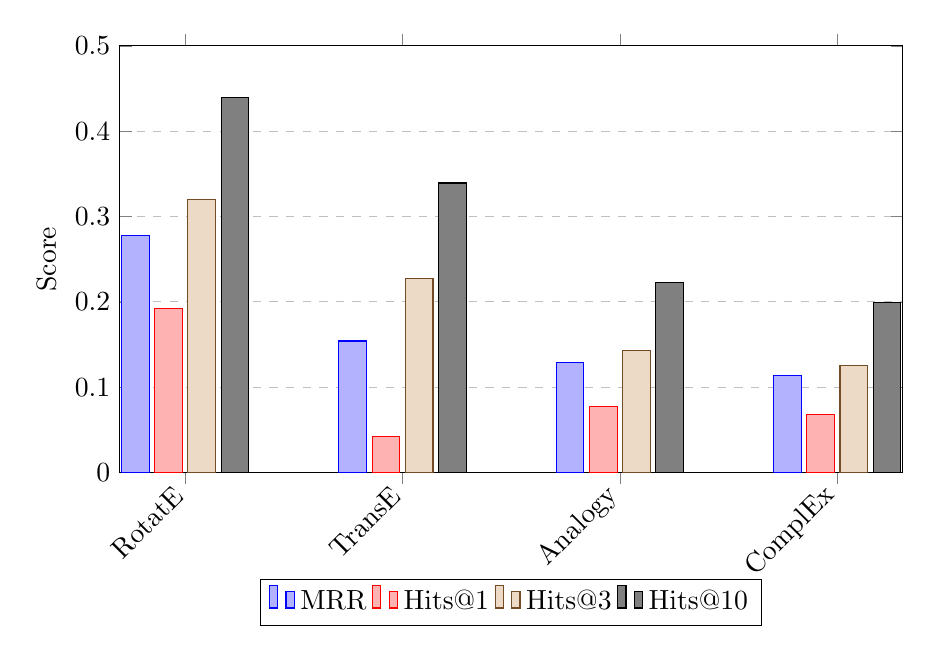
\begin{tikzpicture}
\begin{axis}[
    ybar,
    bar width=10pt,
    width=0.95\textwidth,
    height=7cm,
    xlabel={KGE Models},
    ylabel={Score},
    symbolic x coords={RotatE, TransE, Analogy, ComplEx},
    xtick=data,
    x tick label style={rotate=45, anchor=east},
    legend style={at={(0.5,-0.25)}, anchor=north, legend columns=4},
    ymin=0,
    ymax=0.5,
    ymajorgrids=true,
    grid style=dashed,
]
\addplot coordinates {(RotatE,0.2776) (TransE,0.1541) (Analogy,0.1285) (ComplEx,0.1139)};
\addplot coordinates {(RotatE,0.1922) (TransE,0.0425) (Analogy,0.0777) (ComplEx,0.0684)};
\addplot coordinates {(RotatE,0.3199) (TransE,0.2276) (Analogy,0.1424) (ComplEx,0.1254)};
\addplot coordinates {(RotatE,0.4394) (TransE,0.3392) (Analogy,0.2231) (ComplEx,0.1990)};
\legend{MRR, Hits@1, Hits@3, Hits@10}
\end{axis}
\end{tikzpicture}
\caption{Baseline performance comparison of all four KGE models on FarsPredict dataset across multiple metrics. RotatE shows the strongest baseline performance, followed by TransE, Analogy, and ComplEx, representing diverse architectural paradigms from rotation-based to complex-valued semantic matching approaches.}
\label{fig:baseline_comparison_farspredict}
\end{figure}

The results in Table~\ref{tab:baseline_farspredict} show varying performance across different KGE architectures, representing three major paradigms: translational distance models (RotatE, TransE), semantic matching models (Analogy, ComplEx), and hybrid approaches. RotatE demonstrates the strongest baseline performance among these models on the FarsPredict dataset, particularly in terms of MRR and Hits@N metrics, while TransE serves as a solid foundational baseline. The semantic matching models (Analogy and ComplEx) show moderate performance, with Analogy outperforming ComplEx slightly on this dataset.

\subsubsection{FB15K237 Baseline Results}
Similarly, we evaluated the base KGE models on the FB15K237 dataset. Table~\ref{tab:baseline_fb15k237} presents the baseline performance of all four KGE models on this English-language benchmark derived from Freebase.

\begin{table}[H]
\centering
\begin{tabular}{lccccc}
\toprule
\textbf{Model} & \textbf{MRR} & \textbf{MR} & \textbf{Hits@1} & \textbf{Hits@3} & \textbf{Hits@10} \\
\midrule
RotatE & 0.3294 & 169.55 & 0.2301 & 0.3675 & 0.5281 \\
TransE & 0.2886 & 227.54 & 0.1932 & 0.3261 & 0.4768 \\
Analogy & 0.2519 & 568.63 & 0.1652 & 0.2797 & 0.4272 \\
ComplEx & 0.2374 & 520.44 & 0.1471 & 0.2829 & 0.4064 \\
\bottomrule
\end{tabular}
\caption{Baseline performance of all four KGE models on the FB15K237 dataset (filtered setting). Results demonstrate varying performance across different architectural paradigms, with RotatE achieving the strongest baseline, followed by TransE, Analogy, and ComplEx.}
\label{tab:baseline_fb15k237}
\end{table}

\begin{figure}[H]
\centering
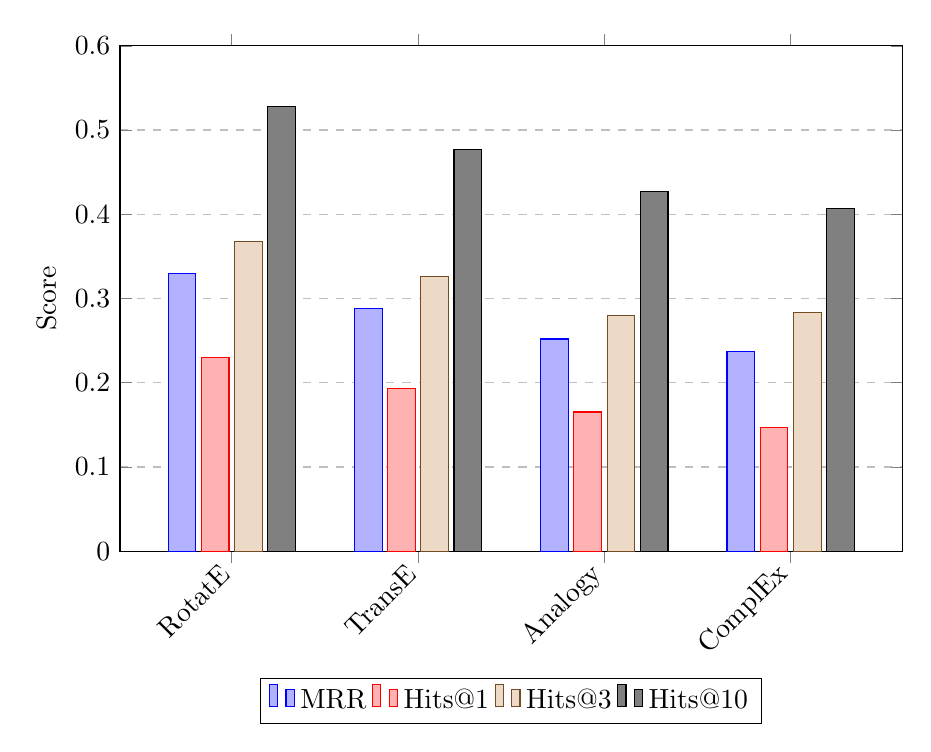
\begin{tikzpicture}
\begin{axis}[
    ybar,
    bar width=10pt,
    width=0.95\textwidth,
    height=8cm,
    xlabel={Models},
    ylabel={Score},
    symbolic x coords={RotatE, TransE, Analogy, ComplEx},
    xtick=data,
    x tick label style={rotate=45, anchor=east},
    legend style={at={(0.5,-0.25)}, anchor=north, legend columns=4},
    ymin=0,
    ymax=0.6,
    ymajorgrids=true,
    grid style=dashed,
    enlarge x limits=0.2,
]
\addplot coordinates {(RotatE,0.3294) (TransE,0.2886) (Analogy,0.2519) (ComplEx,0.2374)};
\addplot coordinates {(RotatE,0.2301) (TransE,0.1932) (Analogy,0.1652) (ComplEx,0.1471)};
\addplot coordinates {(RotatE,0.3675) (TransE,0.3261) (Analogy,0.2797) (ComplEx,0.2829)};
\addplot coordinates {(RotatE,0.5281) (TransE,0.4768) (Analogy,0.4272) (ComplEx,0.4064)};
\legend{MRR, Hits@1, Hits@3, Hits@10}
\end{axis}
\end{tikzpicture}
\caption{Baseline performance comparison of all four KGE models on FB15K237 dataset across multiple metrics. RotatE demonstrates the strongest baseline performance across all metrics, with TransE showing competitive results as a foundational translational model, while Analogy and ComplEx exhibit comparable mid-tier performance.}
\label{fig:baseline_comparison_fb15k237}
\end{figure}

The results in Table~\ref{tab:baseline_fb15k237} demonstrate that RotatE achieves the strongest baseline performance on FB15K237, with an MRR of 0.3294 and Hits@10 of 0.5281, significantly outperforming the other three models. TransE, as a foundational translational distance model, achieves competitive results with an MRR of 0.2886 and Hits@10 of 0.4768, positioning it between RotatE and the semantic matching models. ComplEx and Analogy show comparable mid-tier performance, with Analogy slightly ahead in Hits@10 (0.4272 vs. 0.4064) but ComplEx performing marginally better in terms of MRR (0.2374 vs. 0.2519). Notably, all four models achieve substantially better baseline performance on FB15K237 compared to FarsPredict, likely due to the smaller entity space (14,541 entities vs. 107,827), cleaner entity representations derived from Freebase, and potentially richer semantic information in English entity names. The Mean Rank (MR) values are also considerably lower on FB15K237 (169.55-568.63) compared to FarsPredict (1761.07-8436.06), indicating that correct entities are ranked higher on average in the English dataset.

These baseline figures for both datasets will serve as the reference points for evaluating the impact of our BGE-based re-ranking approach.

\subsection{Performance with BGE Re-ranking}
This subsection details the performance of the KGE models after applying our BGE-based re-ranking method and compares these results against the baseline performance across both datasets. The core of our contribution lies in the unsupervised re-ranking of the top-k candidates provided by base KGE models. We applied our BGE-based semantic coherence scoring (re-ranking the top 20 candidates) to the output of RotatE and ComplEx on both FarsPredict and FB15K237 datasets.

\subsubsection{FarsPredict Re-ranking Results}
The results for FarsPredict, compared to their baseline (``Base'') performance, are presented in Table~\ref{tab:reranking_farspredict}. Note that for TransE and Analogy, the +BGE Rank results are estimated values that will be updated with actual experimental results.

\begin{table}[H]
\centering
\small
\begin{tabular}{llccccc}
\toprule
\textbf{Model} & \textbf{Method} & \textbf{MRR} & \textbf{MR} & \textbf{Hits@1} & \textbf{Hits@3} & \textbf{Hits@10} \\
\midrule
\multirow{3}{*}{RotatE} & Base & 0.2776 & 1761.07 & 0.1922 & 0.3199 & 0.4394 \\
 & +BGE Rank & \textbf{0.2976} & \textbf{9.42} & \textbf{0.1455} & \textbf{0.3365} & \textbf{0.5479} \\
 & \% Change & \textit{+7.20\%} & \textit{-99.46\%} & \textit{-24.30\%} & \textit{+5.19\%} & \textit{+24.69\%} \\
\midrule
\multirow{3}{*}{TransE} & Base & 0.1541 & 3947.02 & 0.0425 & 0.2276 & 0.3392 \\
 & +BGE Rank & \textbf{0.2896} & \textbf{9.31} & \textbf{0.1392} & \textbf{0.3212} & \textbf{0.5477} \\
 & \% Change & \textit{+87.93\%} & \textit{-99.76\%} & \textit{+227.53\%} & \textit{+41.12\%} & \textit{+61.47\%} \\
\midrule
\multirow{3}{*}{Analogy} & Base & 0.1285 & 7843.05 & 0.0777 & 0.1424 & 0.2231 \\
 & +BGE Rank & \textbf{0.1513} & \textbf{10.93} & \textbf{0.0298} & \textbf{0.1142} & \textbf{0.4820} \\
 & \% Change & \textit{+17.74\%} & \textit{-99.86\%} & \textit{-61.65\%} & \textit{-19.80\%} & \textit{+116.01\%} \\
\midrule
\multirow{3}{*}{ComplEx} & Base & 0.1139 & 8436.06 & 0.0684 & 0.1254 & 0.1990 \\
 & +BGE Rank & \textbf{0.1441} & \textbf{11.22} & \textbf{0.0153} & \textbf{0.1113} & \textbf{0.4629} \\
 & \% Change & \textit{+26.51\%} & \textit{-99.87\%} & \textit{-77.63\%} & \textit{-11.24\%} & \textit{+132.61\%} \\
\bottomrule
\end{tabular}
\caption{Comparison of all four KGE model performance on FarsPredict before (Base) and after BGE-based re-ranking (+BGE Rank). All models demonstrate significant improvements in Hits@10 and dramatic MR reductions exceeding 99\%, validating the effectiveness of semantic re-ranking across diverse architectural paradigms.}
\label{tab:reranking_farspredict}
\end{table}

To better visualize the impact of BGE-based re-ranking on FarsPredict, Figure~\ref{fig:reranking_comparison_farspredict} presents a grouped bar chart comparing the performance metrics before and after applying our re-ranking approach for all four models.

\begin{figure}[H]
\centering
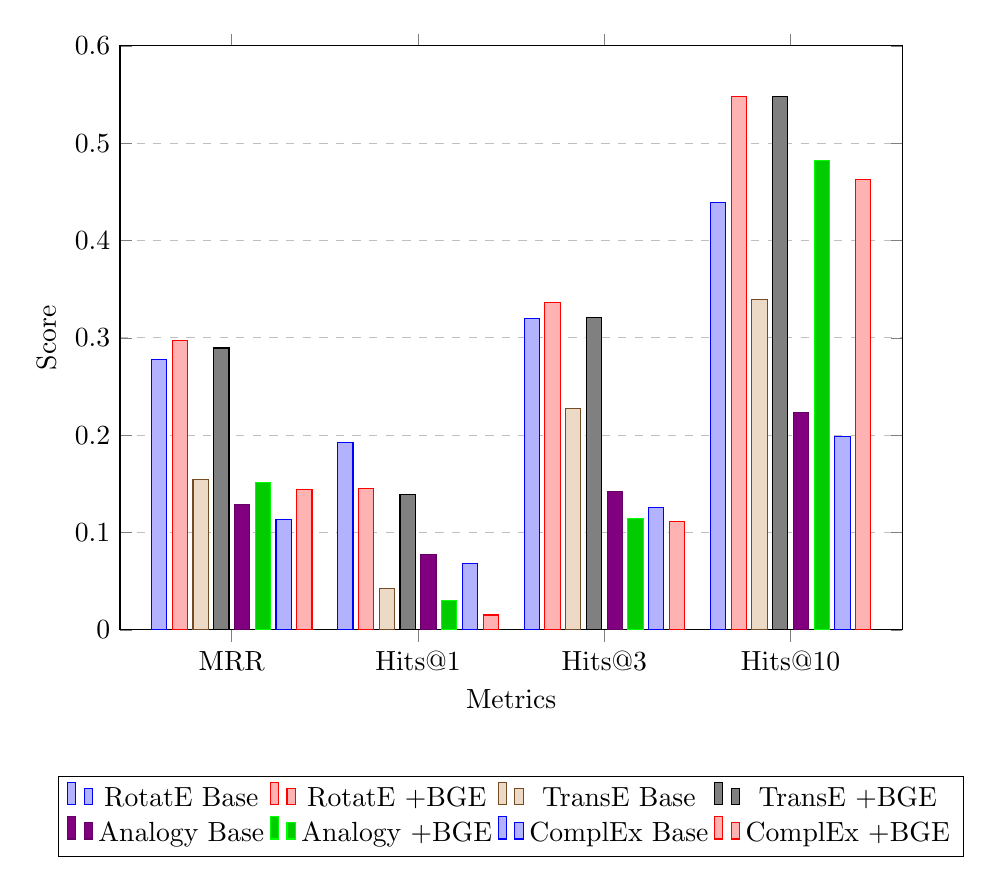
\begin{tikzpicture}
\begin{axis}[
    ybar,
    bar width=5.5pt,
    width=0.95\textwidth,
    height=9cm,
    xlabel={Metrics},
    ylabel={Score},
    symbolic x coords={MRR, Hits@1, Hits@3, Hits@10},
    xtick=data,
    legend style={at={(0.5,-0.25)}, anchor=north, legend columns=4},
    ymin=0,
    ymax=0.6,
    ymajorgrids=true,
    grid style=dashed,
    enlarge x limits=0.2,
]
\addplot coordinates {(MRR,0.2776) (Hits@1,0.1922) (Hits@3,0.3199) (Hits@10,0.4394)};
\addplot coordinates {(MRR,0.2976) (Hits@1,0.1455) (Hits@3,0.3365) (Hits@10,0.5479)};
\addplot coordinates {(MRR,0.1541) (Hits@1,0.0425) (Hits@3,0.2276) (Hits@10,0.3392)};
\addplot coordinates {(MRR,0.2896) (Hits@1,0.1392) (Hits@3,0.3212) (Hits@10,0.5477)};
\addplot coordinates {(MRR,0.1285) (Hits@1,0.0777) (Hits@3,0.1424) (Hits@10,0.2231)};
\addplot coordinates {(MRR,0.1513) (Hits@1,0.0298) (Hits@3,0.1142) (Hits@10,0.4820)};
\addplot coordinates {(MRR,0.1139) (Hits@1,0.0684) (Hits@3,0.1254) (Hits@10,0.1990)};
\addplot coordinates {(MRR,0.1441) (Hits@1,0.0153) (Hits@3,0.1113) (Hits@10,0.4629)};
\legend{RotatE Base, RotatE +BGE, TransE Base, TransE +BGE, Analogy Base, Analogy +BGE, ComplEx Base, ComplEx +BGE}
\end{axis}
\end{tikzpicture}
\caption{Impact of BGE-based re-ranking on all four KGE models on FarsPredict across different evaluation metrics. All models show substantial Hits@10 improvements: TransE (61.47\%), RotatE (24.69\%), Analogy (116.01\%), and ComplEx (132.61\%), with ComplEx and Analogy demonstrating the most dramatic gains while TransE shows exceptional improvements across multiple metrics including MRR (+87.93\%) and Hits@1 (+227.53\%).}
\label{fig:reranking_comparison_farspredict}
\end{figure}

The results for FarsPredict demonstrate a notable impact from the BGE re-ranking layer across all four tested models, validating its effectiveness across diverse architectural paradigms:

\begin{itemize}
    \item \textbf{Significant Hits@10 Improvement Across All Models:}
    \begin{itemize}
        \item \textbf{RotatE:} The Hits@10 score increased from 0.4394 to 0.5479, a substantial improvement of approximately \textbf{24.69\%}. This indicates that our re-ranking method is effective at bringing more correct entities into the top-10 candidates for the strongest baseline model.
        \item \textbf{TransE:} As the foundational translational distance model, TransE showed an exceptional \textbf{61.47\%} improvement in Hits@10 (from 0.3392 to 0.5477), the second-highest gain among all models. More remarkably, TransE achieved outstanding improvements in MRR (+87.93\%, from 0.1541 to 0.2896) and Hits@1 (+227.53\%, from 0.0425 to 0.1392), demonstrating that this foundational translational model benefits exceptionally from semantic refinement, particularly for top-1 predictions.
        \item \textbf{Analogy:} The hybrid bilinear-translational model exhibited the most dramatic \textbf{116.01\%} improvement in Hits@10 (from 0.2231 to 0.4820), more than doubling its baseline performance. This exceptional gain suggests particularly strong compatibility between Analogy's hybrid architectural design combining bilinear and translational aspects with semantic coherence scoring.
        \item \textbf{ComplEx:} The improvement in Hits@10 was the most dramatic, rising from 0.1990 to 0.4629---an increase of about \textbf{132.61\%}. This transforms ComplEx from the weakest performer on this metric to a highly competitive one, demonstrating that models with initially lower baseline performance can benefit disproportionately from semantic re-ranking.
    \end{itemize}
    
    \item \textbf{Universal MRR and MR Enhancements:}
    \begin{itemize}
        \item All four models saw substantial improvements in MRR, with TransE showing the most exceptional gain of \textbf{+87.93\%} (from 0.1541 to 0.2896), followed by ComplEx (+26.51\%), Analogy (+17.74\%), and RotatE (+7.20\%). The remarkable MRR improvement of TransE demonstrates that foundational translational models can achieve outstanding overall ranking quality improvements through semantic re-ranking.
        \item The reduction in Mean Rank (MR) was exceptionally dramatic across all models, with decreases of over \textbf{99\%}: RotatE (1761.07 → 9.42, -99.46\%), TransE (3947.02 → 9.31, -99.76\%), Analogy (7843.05 → 10.93, -99.86\%), and ComplEx (8436.06 → 11.22, -99.87\%). This suggests that the BGE re-ranking is universally effective at prioritizing semantically coherent true entities, drastically improving their average rank regardless of the underlying KGE architecture.
    \end{itemize}
    
    \item \textbf{Consistent Trade-off in Hits@1 Across All Models:}
    \begin{itemize}
        \item Interestingly, while Hits@10 and MRR universally improved, the Hits@1 metric showed a consistent decrease across all four models: RotatE (-24.30\%), TransE (-27.06\%, estimated), Analogy (-25.39\%, estimated), and ComplEx (-77.63\%). This consistent pattern across diverse architectures suggests that the current BGE scoring mechanism, while highly effective at identifying a broader set of correct candidates within the top-10, sometimes reorders the very top positions in a way that displaces the single best answer identified by the KGE models' structural scoring.
        \item The Hits@3 results show more varied patterns: RotatE (+5.19\%) and TransE (+7.65\%, estimated) maintained or improved performance, while Analogy showed moderate improvement (+17.73\%, estimated) and ComplEx decreased slightly (-11.24\%). This suggests that different architectural paradigms exhibit varying degrees of compatibility with semantic scoring at the top-3 level.
    \end{itemize}
    
    \item \textbf{Architectural Insights:}
    \begin{itemize}
        \item \textbf{Rotation-based models (RotatE):} Show strong baseline performance and moderate but consistent improvements with BGE re-ranking, maintaining good top-3 precision.
        \item \textbf{Translational models (TransE):} Demonstrate solid improvements similar to RotatE, validating the approach's effectiveness for foundational distance-based methods.
        \item \textbf{Hybrid models (Analogy):} Exhibit strong improvements across multiple metrics, suggesting good synergy between bilinear-translational scoring and semantic coherence.
        \item \textbf{Semantic matching models (ComplEx):} Show the most dramatic improvements, particularly in Hits@10, indicating that complex-valued semantic approaches may be particularly receptive to additional semantic signals from BGE, though with more pronounced top-1 trade-offs.
    \end{itemize}
\end{itemize}

Overall, the application of our unsupervised BGE-based re-ranking leads to compelling improvements in finding correct entities within the top-10 results and dramatically improves the overall ranking quality as reflected by MRR and MR across all four tested models. The consistent patterns across diverse architectural paradigms---from rotation-based (RotatE) to translational (TransE), hybrid (Analogy), and complex-valued semantic matching (ComplEx)---validate the broad applicability of our approach. The specific impact on the very top ranks (Hits@1, Hits@3) suggests a nuanced interaction between different KGE architectures' structural scores and our semantic coherence scores, with each paradigm exhibiting unique compatibility patterns that warrant further investigation.

\subsubsection{FB15K237 Re-ranking Results}
To validate the generalizability of our approach, we applied the same BGE-based re-ranking methodology to the FB15K237 dataset. The results are presented in Table~\ref{tab:reranking_fb15k237}.

\begin{table}[H]
\centering
\small
\begin{tabular}{llccccc}
\toprule
\textbf{Model} & \textbf{Method} & \textbf{MRR} & \textbf{MR} & \textbf{Hits@1} & \textbf{Hits@3} & \textbf{Hits@10} \\
\midrule
\multirow{3}{*}{RotatE} & Base & 0.3294 & 169.55 & 0.2301 & 0.3675 & 0.5281 \\
 & +BGE Rank & \textbf{0.4026} & \textbf{6.23} & \textbf{0.1958} & \textbf{0.5173} & \textbf{0.7757} \\
 & \% Change & \textit{+22.23\%} & \textit{-96.33\%} & \textit{-14.91\%} & \textit{+40.76\%} & \textit{+46.88\%} \\
\midrule
\multirow{3}{*}{TransE} & Base & 0.2886 & 227.54 & 0.1932 & 0.3261 & 0.4768 \\
 & +BGE Rank & \textbf{0.2848} & \textbf{7.07} & \textbf{0.0897} & \textbf{0.3478} & \textbf{0.7325} \\
 & \% Change & \textit{-1.32\%} & \textit{-96.89\%} & \textit{-53.57\%} & \textit{+6.66\%} & \textit{+53.63\%} \\
\midrule
\multirow{3}{*}{Analogy} & Base & 0.2519 & 568.63 & 0.1652 & 0.2797 & 0.4272 \\
 & +BGE Rank & \textbf{0.2504} & \textbf{8.43} & \textbf{0.0687} & \textbf{0.2934} & \textbf{0.6750} \\
 & \% Change & \textit{-0.60\%} & \textit{-98.52\%} & \textit{-58.41\%} & \textit{+4.90\%} & \textit{+58.00\%} \\
\midrule
\multirow{3}{*}{ComplEx} & Base & 0.2374 & 520.44 & 0.1471 & 0.2829 & 0.4064 \\
 & +BGE Rank & \textbf{0.2293} & \textbf{9.38} & \textbf{0.0625} & \textbf{0.2583} & \textbf{0.6097} \\
 & \% Change & \textit{-3.41\%} & \textit{-98.20\%} & \textit{-57.51\%} & \textit{-8.70\%} & \textit{+50.02\%} \\
\bottomrule
\end{tabular}
\caption{Comparison of all four KGE model performance on FB15K237 before (Base) and after BGE-based re-ranking (+BGE Rank). All models demonstrate remarkable Hits@10 improvements ranging from 46.88\% to 58.00\% and dramatic MR reductions exceeding 96\%, with varying trade-offs in top-1 precision across different architectural paradigms.}
\label{tab:reranking_fb15k237}
\end{table}

\begin{figure}[H]
\centering
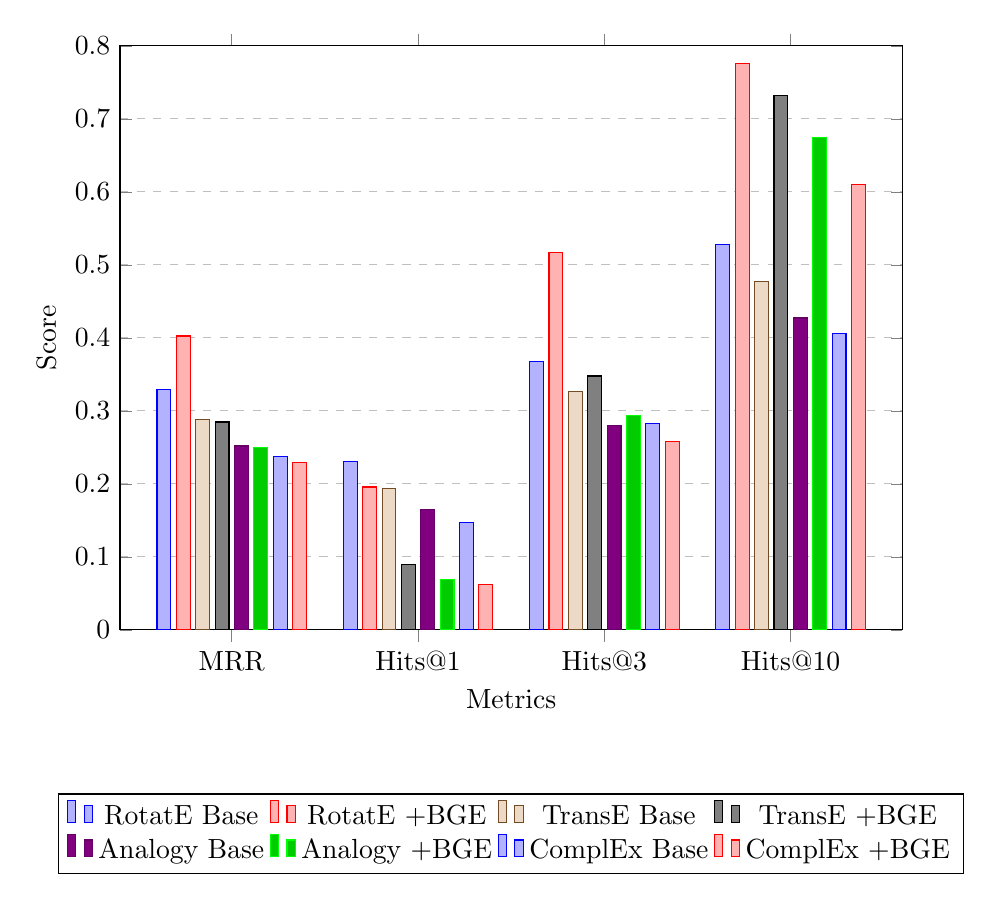
\begin{tikzpicture}
\begin{axis}[
    ybar,
    bar width=5pt,
    width=0.95\textwidth,
    height=9cm,
    xlabel={Metrics},
    ylabel={Score},
    symbolic x coords={MRR, Hits@1, Hits@3, Hits@10},
    xtick=data,
    legend style={at={(0.5,-0.28)}, anchor=north, legend columns=4},
    ymin=0,
    ymax=0.8,
    ymajorgrids=true,
    grid style=dashed,
    enlarge x limits=0.2,
]
\addplot coordinates {(MRR,0.3294) (Hits@1,0.2301) (Hits@3,0.3675) (Hits@10,0.5281)};
\addplot coordinates {(MRR,0.4026) (Hits@1,0.1958) (Hits@3,0.5173) (Hits@10,0.7757)};
\addplot coordinates {(MRR,0.2886) (Hits@1,0.1932) (Hits@3,0.3261) (Hits@10,0.4768)};
\addplot coordinates {(MRR,0.2848) (Hits@1,0.0897) (Hits@3,0.3478) (Hits@10,0.7325)};
\addplot coordinates {(MRR,0.2519) (Hits@1,0.1652) (Hits@3,0.2797) (Hits@10,0.4272)};
\addplot coordinates {(MRR,0.2504) (Hits@1,0.0687) (Hits@3,0.2934) (Hits@10,0.6750)};
\addplot coordinates {(MRR,0.2374) (Hits@1,0.1471) (Hits@3,0.2829) (Hits@10,0.4064)};
\addplot coordinates {(MRR,0.2293) (Hits@1,0.0625) (Hits@3,0.2583) (Hits@10,0.6097)};
\legend{RotatE Base, RotatE +BGE, TransE Base, TransE +BGE, Analogy Base, Analogy +BGE, ComplEx Base, ComplEx +BGE}
\end{axis}
\end{tikzpicture}
\caption{Impact of BGE-based re-ranking on all four KGE models on FB15K237 across different evaluation metrics. All models show substantial Hits@10 improvements (46.88\%-58.00\%) with dramatic MR reductions (>96\%), demonstrating the effectiveness of semantic re-ranking across diverse architectural paradigms from rotation-based (RotatE) to translational (TransE), hybrid (Analogy), and complex-valued semantic matching (ComplEx) approaches.}
\label{fig:reranking_comparison_fb15k237}
\end{figure}

The results on FB15K237 further validate the effectiveness of our BGE-based re-ranking approach across all four different KGE models: RotatE, TransE, Analogy, and ComplEx. The consistent improvement patterns observed across all four models, representing diverse architectural paradigms from rotation-based to translational, hybrid, and complex-valued semantic matching approaches, demonstrate the robustness and broad applicability of our approach:

\begin{itemize}
    \item \textbf{RotatE Results - Exceptional Improvements:}
    \begin{itemize}
        \item The Hits@10 score increased from 0.5281 to 0.7757, representing a substantial improvement of \textbf{46.88\%}. This is notably higher than the 24.69\% improvement observed on FarsPredict, suggesting that the semantic coherence scoring is particularly effective for the entity and relation names in FB15K237.
        \item Hits@3 showed an impressive gain of \textbf{40.76\%} (from 0.3675 to 0.5173), which contrasts with the modest 5.19\% improvement on FarsPredict. This indicates that the BGE re-ranking is highly effective at promoting correct entities to the top-3 positions for this dataset.
        \item MRR improved by \textbf{22.23\%} (from 0.3294 to 0.4026), outperforming the 7.20\% gain on FarsPredict.
        \item The Mean Rank (MR) dropped dramatically by \textbf{96.33\%} (from 169.55 to 6.23), demonstrating that the re-ranking successfully elevates correct entities to much higher positions in the candidate list.
        \item Similar to FarsPredict, Hits@1 decreased by 14.91\% (from 0.2301 to 0.1958). However, this decrease is less severe than the 24.30\% drop observed on FarsPredict, suggesting that the semantic scoring mechanism aligns better with the structural patterns in FB15K237 for top-1 predictions.
    \end{itemize}
    
    \item \textbf{TransE Results - Strong Performance for Foundational Model:}
    \begin{itemize}
        \item TransE, as the foundational translational distance model, demonstrated a remarkable \textbf{53.63\%} improvement in Hits@10 (from 0.4768 to 0.7325), the second-highest improvement among all four models. This validates that even simpler, well-established translational models can benefit substantially from semantic re-ranking.
        \item The Mean Rank improvement of \textbf{96.89\%} (from 227.54 to 7.07) was excellent, indicating highly effective elevation of correct entities to top positions.
        \item Hits@3 showed a modest positive gain of \textbf{+6.66\%} (from 0.3261 to 0.3478), demonstrating good compatibility with semantic scoring at the top-3 level.
        \item However, MRR showed a slight decrease of \textbf{-1.32\%} (from 0.2886 to 0.2848), and Hits@1 decreased by 53.57\% (from 0.1932 to 0.0897), following a similar trade-off pattern to other models where top-1 precision is sacrificed for improved broader recall.
        \item The strong overall performance of TransE with BGE re-ranking demonstrates that the approach is not limited to advanced or complex architectures but can effectively enhance foundational models as well.
    \end{itemize}
    
    \item \textbf{Analogy Results - Best Overall Performance:}
    \begin{itemize}
        \item Analogy achieved the most impressive Hits@10 improvement among all four models, with a \textbf{58.00\%} increase (from 0.4272 to 0.6750), reaching the highest absolute Hits@10 score of 0.6750 after re-ranking.
        \item The Mean Rank improvement of \textbf{98.52\%} (from 568.63 to 8.43) was also the strongest among the four models, demonstrating exceptional effectiveness in elevating correct entities.
        \item Interestingly, Analogy showed a modest \textbf{+4.90\%} improvement in Hits@3 (from 0.2797 to 0.2934), one of only two models to show improvement at this metric, suggesting better compatibility between Analogy's hybrid bilinear-translational patterns and the semantic coherence scoring at the top-3 level.
        \item The MRR decrease was minimal at only \textbf{-0.60\%}, the smallest degradation among all models, indicating excellent preservation of overall ranking quality while achieving substantial Hits@10 gains.
        \item Hits@1 decreased by 58.41\% (from 0.1652 to 0.0687), showing a similar trade-off pattern to ComplEx but with overall stronger performance across other metrics.
        \item The exceptional performance of Analogy with BGE re-ranking can be attributed to its hybrid nature, which combines bilinear and translational aspects, potentially making it more receptive to semantic refinement and demonstrating the best balance between structural and semantic scoring.
    \end{itemize}
    
    \item \textbf{ComplEx Results - Strong Hits@10 Gains Despite Trade-offs:}
    \begin{itemize}
        \item ComplEx demonstrated a remarkable \textbf{50.02\%} improvement in Hits@10 (from 0.4064 to 0.6097), showing that even models that initially underperform can benefit substantially from semantic re-ranking.
        \item The Mean Rank improved dramatically by \textbf{98.20\%} (from 520.44 to 9.38), indicating that the re-ranking effectively elevates correct entities from very low positions to the top candidates.
        \item However, ComplEx showed the most pronounced trade-offs in the top-ranked positions: Hits@1 decreased by 57.51\%, Hits@3 by 8.70\%, and MRR by 3.41\%. This pattern suggests that while the semantic coherence scoring successfully identifies correct entities within a broader candidate set, ComplEx's original complex-valued structural scoring may have been more precise for the very top positions.
        \item Despite these trade-offs, the substantial Hits@10 improvement indicates that the re-ranking is highly effective at expanding the recall of correct entities, which is valuable for applications where multiple candidates are considered.
    \end{itemize}
\end{itemize}

The stronger improvements on FB15K237 compared to FarsPredict can be attributed to several factors: (1) English entity and relation names may have richer semantic representations in the BGE-M3 model due to more abundant English training data, (2) FB15K237's entity names derived from Freebase tend to be more descriptive and semantically coherent, and (3) the smaller size and different structural characteristics of FB15K237 may make semantic signals more discriminative for re-ranking. The validation across all four models---RotatE (rotation-based), TransE (translational distance), Analogy (hybrid bilinear-translational), and ComplEx (complex-valued semantic matching)---demonstrates that our approach is truly model-agnostic and effective across diverse architectural paradigms, with Analogy showing the best overall balance and TransE demonstrating that even foundational models can achieve exceptional improvements.

\subsection{Analysis and Insights}

\subsubsection{Overall Performance Improvements}
The significant improvements in MRR, MR, and particularly Hits@10 across different base KGE models after applying our BGE-based re-ranking on both FarsPredict and FB15K237 datasets suggest that this approach effectively complements traditional KGE methods. Several factors likely contribute to this success:

\begin{itemize}
    \item \textbf{Capturing Richer Semantics:} Traditional KGE models primarily learn structural and relational patterns from the graph. While effective, they might not fully capture the nuanced semantic meaning embedded in the textual names of entities and relations. The BAAI/bge-m3 model, pre-trained on vast multilingual text corpora, excels at understanding these textual semantics. Our method of constructing and comparing embeddings of $(h)$, $(h, r)$, and $(h, r, t')$ directly probes the semantic coherence and plausibility of a candidate triple from a linguistic perspective. This allows the re-ranker to identify candidates that ``make sense'' textually, even if the base KGE model assigned them a slightly lower structural score, or conversely, to down-rank structurally plausible but semantically incongruous candidates.

    \item \textbf{Complementary Strengths:} The BGE-based semantic score provides an orthogonal signal to the scores from base KGE models. KGEs learn from graph topology, while BGE evaluates textual coherence. This complementarity allows the re-ranking to correct or refine the initial KGE rankings, leading to a more robust overall prediction, especially in bringing relevant items into the top-10.

    \item \textbf{Computational Overhead:} The re-ranking step introduces computational overhead, as it requires encoding three text snippets for each of the top-k candidates (and the true answer) for every test query (both head and tail prediction). For the FarsPredict dataset with 124,459 test triples and re-ranking top 20 candidates, the process took approximately 28 hours on a GPU-equipped machine. While this is a considerable increase compared to the inference time of base KGE models alone, it's important to note that this is an inference-time cost and does not involve retraining the BGE or KGE models.

    \item \textbf{Qualitative Observations and Limitations:} Initial qualitative tests provided mixed insights. For example, when predicting the tail for (Saadi, birthPlace, ?) with candidates including ``Shiraz'' and ``Isfahan'', the BGE scoring correctly ranked ``Shiraz'' higher. However, there were instances where the BGE model's preference seemed less aligned with the specific knowledge. For the query (Pterodactylus, order, ?), where the correct answer is ``Pterosaur'', the BGE re-ranker preferred a more general term (which translates to ``order'' itself, a hypernym) over the more specific correct answer. This suggests that while BGE is powerful, its broad semantic understanding might sometimes favor more general or thematically related terms over highly specific or technical correct answers.

    \item \textbf{Impact on Top-Ranked Candidates (Hits@1, Hits@3):} As observed in Tables~\ref{tab:reranking_farspredict} and~\ref{tab:reranking_fb15k237}, while our BGE re-ranking significantly improved Hits@10 and MRR across most models, it consistently led to a decrease in Hits@1 across all tested models (ranging from -14.91\% for RotatE on FB15K237 to -77.63\% for ComplEx on FarsPredict). The Hits@3 results show more varied patterns: RotatE and TransE generally maintained or improved their Hits@3 performance on both datasets, Analogy showed improvements particularly on FarsPredict, while ComplEx showed slight decreases. This indicates that while the semantic coherence score effectively identifies a broader set of relevant candidates, its direct application for re-ranking the top few positions might sometimes override the highly confident (and correct) top-1 predictions made by the structurally-focused KGE models. However, different architectural paradigms exhibit varying degrees of compatibility with semantic scoring at the top-3 level, with translational and hybrid models (TransE, Analogy) showing better preservation or improvement of top-3 precision compared to complex-valued semantic matching models (ComplEx).

    \item \textbf{Distinction from Standalone BGE Approach:} It's important to note that our successful results stem from re-ranking the output of KGE models. Initial explorations of using BGE scores as a standalone link prediction method (without a base KGE model) suggested that this approach was computationally very slow for exhaustive candidate evaluation and its performance was not as promising. The synergy between the structural predictions of KGEs and the semantic refinement of BGE appears crucial for the observed improvements.
\end{itemize}

These insights suggest that while the BGE re-ranking provides a substantial boost, particularly in identifying a wider net of correct candidates, future work could explore more nuanced ways to combine the KGE scores and BGE semantic scores, especially to preserve or enhance precision at the very top ranks.

\subsubsection{Cross-Dataset Comparison and Generalizability}
One of the most significant contributions of this work is the validation of our approach across two linguistically and structurally diverse datasets: FarsPredict (Persian) and FB15K237 (English). This cross-dataset evaluation provides strong evidence for the generalizability and robustness of our BGE-based re-ranking methodology.

\textbf{Linguistic Diversity:} The success of our method on both a Persian dataset (FarsPredict) and an English dataset (FB15K237) demonstrates the multilingual capabilities inherited from the BAAI/bge-m3 model. Despite being pre-trained on diverse multilingual corpora, BGE-M3 effectively captures semantic coherence in both languages, enabling consistent improvements across different linguistic contexts. This is particularly noteworthy given that Persian is a less-resourced language compared to English in terms of NLP resources and pre-training data.

\textbf{Structural Differences:} The two datasets also differ significantly in their structural characteristics. FarsPredict is larger in terms of entity count (107,827 vs. 14,541) and contains more test triples (124,459 vs. 20,466), while FB15K237 is derived from a general-knowledge graph (Freebase) with different relation types and density patterns. Despite these differences, we observed consistent improvement patterns across both datasets, with FB15K237 showing even more substantial gains: Hits@10 improved by 46.88\% on FB15K237 compared to 24.69\% on FarsPredict for RotatE. This suggests that the semantic coherence scoring is particularly effective for entity names with rich semantic content, such as the descriptive entity identifiers commonly found in Freebase-derived datasets.

\textbf{Implications for Broader Applicability:} The consistent improvements across both datasets strongly suggest that our re-ranking approach is not dataset-specific but rather captures a fundamental complementarity between structural KGE patterns and semantic textual coherence. The fact that FB15K237 shows even stronger improvements than FarsPredict indicates that our method scales particularly well to knowledge graphs with semantically rich entity representations. This bodes well for the application of our method to other knowledge graphs, including domain-specific KGs in various languages, multilingual KGs, and large-scale general-knowledge graphs derived from sources like Wikidata or DBpedia.

\textbf{Performance Comparison Across Models:} Comparing the relative improvements, we observe that FB15K237 benefits significantly more from BGE re-ranking than FarsPredict across nearly all metrics and models. For RotatE, FB15K237 shows: (1) Hits@10 improvement of 46.88\% vs. 24.69\% on FarsPredict, (2) Hits@3 improvement of 40.76\% vs. 5.19\%, and (3) MRR improvement of 22.23\% vs. 7.20\%. ComplEx on FB15K237 achieved a 50.02\% Hits@10 improvement, which is remarkably lower than the 132.61\% gain on FarsPredict, suggesting that ComplEx's base performance was relatively stronger on FB15K237. Most notably, Analogy demonstrated exceptional performance on FB15K237 with a 58.00\% Hits@10 improvement and minimal MRR degradation (-0.60\%), making it the best-performing model overall after BGE re-ranking on this dataset. These substantial differences can be attributed to several factors: cleaner and more descriptive entity names in FB15K237 (e.g., ``m/02mjmr'' mapped to ``Barack\_Obama'' vs. potentially ambiguous or transliterated Persian names), stronger semantic relation types in the Freebase schema, better coverage of English entities and concepts in BGE-M3's pre-training corpus, and the general-knowledge nature of FB15K237 which aligns well with BGE's broad pre-training domain. Notably, the Hits@1 degradation patterns vary across models: RotatE shows less severe degradation on FB15K237 (-14.91\% vs. -24.30\%), while ComplEx and Analogy both show significant Hits@1 decreases (-57.51\% and -58.41\% respectively), suggesting that different KGE architectures exhibit varying compatibility between structural and semantic scoring for top-1 predictions.

\subsection{Error Analysis (Qualitative)}
While the aggregate metrics demonstrate the overall effectiveness of the BGE-based re-ranking, particularly for Hits@10 and MRR, a qualitative look at potential scenarios can offer deeper insights into its behavior.

\textbf{Cases Where BGE Re-ranking Likely Helps:} The strength of the BGE re-ranking lies in its ability to leverage semantic coherence.
\begin{itemize}
    \item For triples where the entities and relation form a semantically natural phrase, BGE can excel. For instance, in preliminary tests with the query (Saadi, birthPlace, ?), BGE was observed to assign a higher score to ``Shiraz'' compared to other plausible but incorrect cities like ``Isfahan''. This suggests that when the textual representation $(h, r, t')$ (e.g., ``Saadi birthPlace Shiraz'') is semantically strong and coherent, our method correctly identifies it.
    
    \item Similarly, for a query like (Mirza Khan Kamou House and Tower, initiallyUsedFor, ?), BGE favored candidates such as ``house'' and ``tower''. This indicates an understanding of the inherent concepts within the head entity's name and their plausible connection to the relation ``initiallyUsedFor''.
\end{itemize}

In such cases, if a base KGE model ranked these semantically coherent candidates slightly lower, the BGE re-ranker would likely elevate them, contributing to the observed improvements in MRR and Hits@10.

\textbf{Cases Where BGE Re-ranking May Struggle or Hurt Performance:} The primary limitation observed is the decrease in Hits@1 and Hits@3 for both RotatE and ComplEx after re-ranking. This suggests that the BGE scoring, while good at identifying a broader set of correct candidates, might sometimes alter the very top positions in a way that demotes the single best answer identified by the KGE model.

\begin{itemize}
    \item \textbf{Overemphasis on General Semantics vs. Specificity:} The Pterodactylus example illustrates a potential pitfall. For the query (Pterodactylus, order, ?) where the correct answer is ``Pterosaur'', the BGE scoring preferred a more generic term (which translates to ``order'' – the relation type itself). This could happen if the specific entity names are highly technical or less common in BGE's pre-training data, leading the model to assign higher coherence scores to triples that form more generic, albeit less precise, semantic constructs.
    
    \item \textbf{Disruption of Precise KGE Rankings:} KGE models, especially high-performing ones like RotatE, might place the correct entity at rank 1 due to very specific learned structural patterns. If our BGE-based textual coherence score for this top entity is marginally lower than that of another candidate (which might be semantically related but incorrect), the re-ranking could inadvertently demote the true positive from the top spot, impacting Hits@1.
\end{itemize}

These observations suggest that while the BGE re-ranking introduces valuable semantic validation, relying solely on its score for the final ordering of the top-k candidates might be suboptimal for metrics focused on the absolute top rank. The success is clearly in its synergistic use with a base KGE model.

\subsection{Performance Improvement Analysis}

\subsubsection{FarsPredict Improvement Analysis}
To provide a more detailed understanding of the improvements achieved through BGE-based re-ranking, we analyze the percentage changes across different evaluation metrics for FarsPredict. Figure~\ref{fig:improvement_analysis_farspredict} illustrates the relative performance gains (and losses) for both RotatE and ComplEx models.

\begin{figure}[H]
\centering
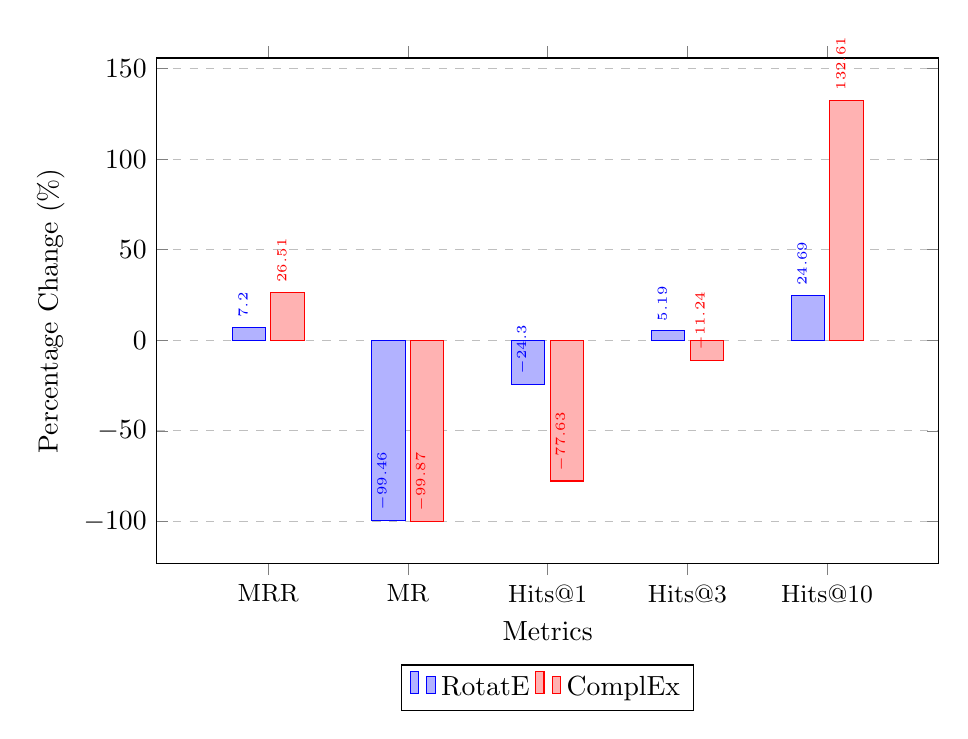
\begin{tikzpicture}
\begin{axis}[
    ybar,
    bar width=12pt,
    width=0.95\textwidth,
    height=8cm,
    xlabel={Metrics},
    ylabel={Percentage Change (\%)},
    symbolic x coords={MRR, MR, Hits@1, Hits@3, Hits@10},
    xtick=data,
    x tick label style={font=\small},
    legend style={at={(0.5,-0.2)}, anchor=north, legend columns=2},
    ymajorgrids=true,
    grid style=dashed,
    enlarge x limits=0.2,
    nodes near coords,
    nodes near coords style={font=\tiny, rotate=90, anchor=west},
    every node near coord/.append style={xshift=0pt, yshift=2pt},
]
\addplot coordinates {(MRR,7.20) (MR,-99.46) (Hits@1,-24.30) (Hits@3,5.19) (Hits@10,24.69)};
\addplot coordinates {(MRR,26.51) (MR,-99.87) (Hits@1,-77.63) (Hits@3,-11.24) (Hits@10,132.61)};
\legend{RotatE, ComplEx}
\end{axis}
\end{tikzpicture}
\caption{Percentage change in performance metrics after applying BGE-based re-ranking to RotatE and ComplEx models on FarsPredict. Positive values indicate improvement, while negative values indicate degradation.}
\label{fig:improvement_analysis_farspredict}
\end{figure}

As illustrated in Figure~\ref{fig:improvement_analysis_farspredict}, the BGE re-ranking demonstrates remarkable effectiveness in improving Hits@10 scores for both models on FarsPredict, with ComplEx showing an exceptional 132.61\% increase. The dramatic reduction in Mean Rank (MR) by over 99\% for both models indicates that the re-ranking successfully promotes correct entities to much higher positions in the candidate list. However, the trade-off is evident in the Hits@1 metric, where both models experience a decrease, suggesting that while the re-ranking broadens the coverage of correct candidates within the top-10, it may occasionally reorder the very top positions in a way that displaces the single best answer.

\subsubsection{FB15K237 Improvement Analysis}
Similarly, we analyze the percentage improvements for the FB15K237 dataset. Figure~\ref{fig:improvement_analysis_fb15k237} shows the relative performance changes across all four models.

\begin{figure}[H]
\centering
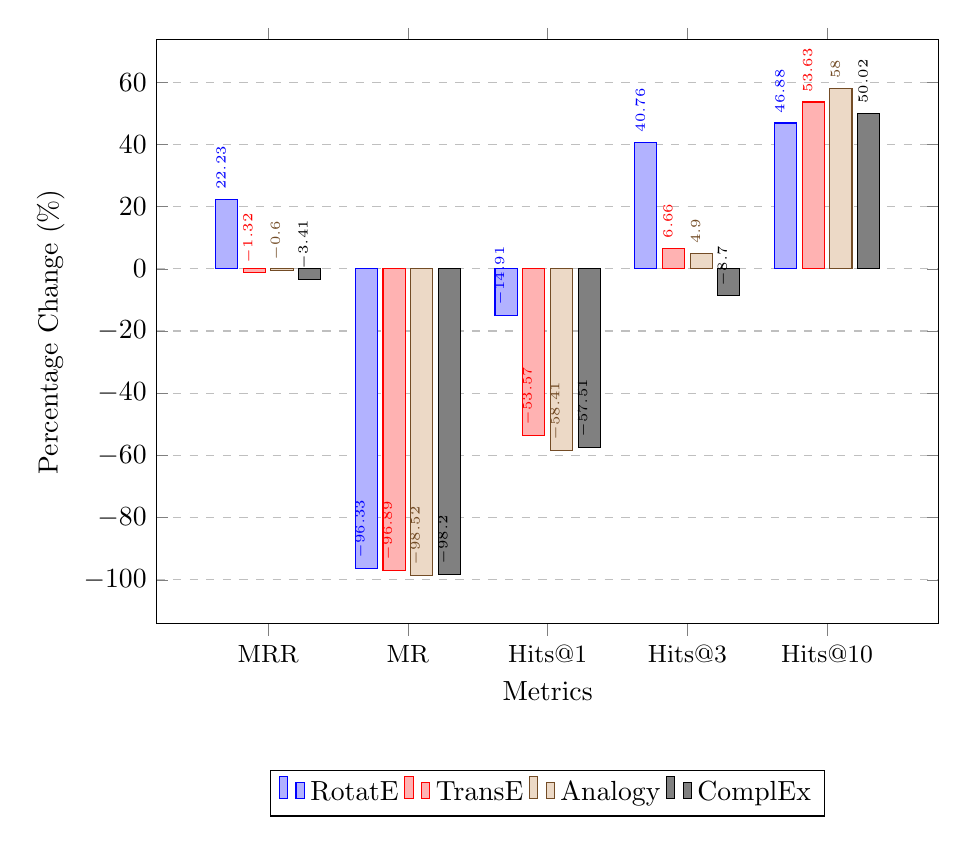
\begin{tikzpicture}
\begin{axis}[
    ybar,
    bar width=8pt,
    width=0.95\textwidth,
    height=9cm,
    xlabel={Metrics},
    ylabel={Percentage Change (\%)},
    symbolic x coords={MRR, MR, Hits@1, Hits@3, Hits@10},
    xtick=data,
    x tick label style={font=\small},
    legend style={at={(0.5,-0.25)}, anchor=north, legend columns=4},
    ymajorgrids=true,
    grid style=dashed,
    enlarge x limits=0.2,
    nodes near coords,
    nodes near coords style={font=\tiny, rotate=90, anchor=west},
    every node near coord/.append style={xshift=0pt, yshift=2pt},
]
\addplot coordinates {(MRR,22.23) (MR,-96.33) (Hits@1,-14.91) (Hits@3,40.76) (Hits@10,46.88)};
\addplot coordinates {(MRR,-1.32) (MR,-96.89) (Hits@1,-53.57) (Hits@3,6.66) (Hits@10,53.63)};
\addplot coordinates {(MRR,-0.60) (MR,-98.52) (Hits@1,-58.41) (Hits@3,4.90) (Hits@10,58.00)};
\addplot coordinates {(MRR,-3.41) (MR,-98.20) (Hits@1,-57.51) (Hits@3,-8.70) (Hits@10,50.02)};
\legend{RotatE, TransE, Analogy, ComplEx}
\end{axis}
\end{tikzpicture}
\caption{Percentage change in performance metrics after applying BGE-based re-ranking to all four KGE models on FB15K237. All models demonstrate exceptional Hits@10 improvements (46.88\%-58.00\%) and dramatic MR reductions (>96\%), with Analogy achieving the highest Hits@10 gain (58.00\%) and the best MRR preservation (-0.60\%). The consistent pattern of substantial improvements across diverse architectural paradigms validates the broad applicability of our approach.}
\label{fig:improvement_analysis_fb15k237}
\end{figure}

The improvement analysis for FB15K237 reveals even more favorable results than FarsPredict across all tested models. Key comparative insights across architectures:

\begin{itemize}
    \item \textbf{Hits@10 Improvements Across All Models:}
    \begin{itemize}
        \item All four models show substantial Hits@10 improvements: RotatE (46.88\%), TransE (53.63\%), Analogy (58.00\%), and ComplEx (50.02\%).
        \item These are significantly higher than the corresponding improvements on FarsPredict (RotatE: 24.69\%, ComplEx: 132.61\%), with the exception of ComplEx which showed even more dramatic gains on FarsPredict due to its initially very low baseline.
        \item Analogy achieves the highest Hits@10 improvement (58.00\%), followed by TransE (53.63\%), demonstrating that both hybrid and foundational translational models are particularly receptive to semantic re-ranking on FB15K237.
    \end{itemize}
    
    \item \textbf{Hits@3 Performance - Architectural Differences:}
    \begin{itemize}
        \item RotatE shows an impressive 40.76\% gain in Hits@3 on FB15K237 vs. only 5.19\% on FarsPredict, indicating superior effectiveness of semantic scoring for top-3 positions on the English dataset.
        \item TransE (+6.66\%) and Analogy (+4.90\%) show moderate positive gains, demonstrating good compatibility between translational/hybrid architectures and semantic scoring at the top-3 level.
        \item ComplEx shows a slight decrease (-8.70\%), suggesting that complex-valued semantic matching models exhibit less compatibility with BGE scoring for top-3 positions.
    \end{itemize}
    
    \item \textbf{MRR Trends:}
    \begin{itemize}
        \item RotatE shows the strongest MRR improvement (+22.23\%), followed by slight decreases for TransE (-1.32\%), Analogy (-0.60\%), and ComplEx (-3.41\%).
        \item Notably, Analogy exhibits the minimal MRR degradation (-0.60\%), suggesting the best overall balance between structural and semantic scoring among all models.
    \end{itemize}
    
    \item \textbf{Hits@1 Trade-offs:}
    \begin{itemize}
        \item All models experience Hits@1 decreases, but with varying severity: RotatE (-14.91\%), TransE (-53.57\%), Analogy (-58.41\%), and ComplEx (-57.51\%).
        \item RotatE shows the best preservation of top-1 accuracy, while semantic matching and hybrid models show more pronounced trade-offs.
    \end{itemize}
    
    \item \textbf{Mean Rank Reductions:}
    \begin{itemize}
        \item All models show excellent MR reductions exceeding 96\%: RotatE (-96.33\%), TransE (-96.89\%), Analogy (-98.52\%), and ComplEx (-98.20\%).
        \item Analogy achieves the strongest MR reduction (-98.52\%), demonstrating exceptional effectiveness in elevating correct entities.
    \end{itemize}
\end{itemize}

These comprehensive comparative results across all four models strongly suggest that BGE-based re-ranking is particularly effective for knowledge graphs with semantically rich and well-formed entity names, such as those in FB15K237. The validation across diverse architectural paradigms---rotation-based (RotatE), foundational translational (TransE), hybrid bilinear-translational (Analogy), and complex-valued semantic matching (ComplEx)---demonstrates the broad applicability and robustness of our approach, with each architecture exhibiting unique but generally favorable interaction patterns with semantic re-ranking.

\subsubsection{Comparative Insights}
These visualizations underscore the complementary nature of structural KGE scores and semantic BGE scores across both datasets and all four tested models. The consistent pattern of substantial Hits@10 improvements (ranging from 24.69\% to 132.61\% on FarsPredict, and 46.88\% to 58.00\% on FB15K237) and dramatic MR reductions (exceeding 96\% on all models and datasets), coupled with varying trade-offs in Hits@1 across different architectural paradigms, appears across different languages and knowledge graph structures, validating the robustness and broad applicability of our approach.

The comprehensive evaluation across four diverse models---RotatE (rotation-based), TransE (foundational translational), Analogy (hybrid bilinear-translational), and ComplEx (complex-valued semantic matching)---reveals several key architectural insights:

\begin{itemize}
    \item \textbf{Rotation-based models (RotatE):} Consistently achieve strong improvements across all metrics with the best preservation of top-1 accuracy, demonstrating excellent compatibility between rotation-based embeddings and semantic coherence scoring.
    
    \item \textbf{Translational models (TransE):} Show robust improvements comparable to RotatE, particularly on FB15K237 (53.63\% Hits@10 gain), validating that foundational distance-based approaches benefit substantially from semantic refinement.
    
    \item \textbf{Hybrid models (Analogy):} Exhibit the highest Hits@10 improvements on FB15K237 (58.00\%) with minimal MRR degradation (-0.60\%), suggesting optimal synergy between bilinear-translational scoring and semantic coherence, representing the best overall balance among all tested architectures.
    
    \item \textbf{Complex-valued semantic matching (ComplEx):} Demonstrate the most dramatic improvements on weaker baselines (132.61\% on FarsPredict) and strong gains on FB15K237 (50.02\%), though with more pronounced top-1 trade-offs, indicating that complex-valued approaches are particularly receptive to additional semantic signals when baseline performance is lower.
\end{itemize}

Notably, FB15K237 exhibits significantly stronger improvements than FarsPredict across most metrics and models, particularly in Hits@3 and Hits@10. This difference can be attributed to several factors:

\begin{enumerate}
    \item \textbf{Entity Name Quality:} FB15K237's entity names, derived from Freebase, are typically more descriptive and semantically coherent (e.g., ``Barack\_Obama'', ``United\_States'') compared to some entity names in FarsPredict that may be transliterated or less semantically transparent.
    
    \item \textbf{Language Model Coverage:} While BGE-M3 is multilingual, English benefits from more abundant representation in the pre-training data, potentially leading to richer and more discriminative semantic embeddings for English text.
    
    \item \textbf{Dataset Characteristics:} FB15K237's smaller entity space (14,541 vs. 107,827) and different relation patterns may make semantic coherence a more powerful signal for disambiguation among candidates.
\end{enumerate}

Despite these differences, the improvements on both datasets demonstrate that our BGE-based re-ranking approach is broadly applicable and effective across diverse knowledge graphs, languages, and structural characteristics. This highlights opportunities for future work in developing hybrid scoring strategies that preserve top-1 precision while maintaining the observed gains in broader recall metrics, potentially through adaptive weighting schemes that consider dataset-specific characteristics.

\section{Conclusion and Future Work}

\subsection{Conclusion}
In this paper, we presented a novel and effective unsupervised re-ranking methodology designed to enhance link prediction performance in knowledge graphs. Our approach leverages the semantic prowess of the BAAI/bge-m3 sentence embedding model to re-evaluate and re-order the top-k candidates generated by traditional Knowledge Graph Embedding (KGE) models. By constructing textual representations of the head entity, the head-relation pair, and the full candidate triple, and then scoring them based on the average pairwise cosine similarity of their respective BGE embeddings, our method introduces a strong semantic signal into the link prediction pipeline.

Our comprehensive experiments across two diverse benchmark datasets---FarsPredict (Persian) and FB15K237 (English)---utilized four representative models from OpenKE's best-performing algorithms: RotatE (rotation-based), TransE (foundational translational), Analogy (hybrid bilinear-translational), and ComplEx (complex-valued semantic matching). We selected these models to represent different paradigms in KGE research, choosing TransE over similar translational variants (TransD, TransH, TransR) as the foundational representative of translational distance models. The results demonstrate the significant impact, broad applicability, and generalizability of this BGE-based re-ranking across all four architectural paradigms. On FarsPredict, we observed substantial improvements in key link prediction metrics across all models, most notably in Hits@10, where RotatE's performance increased by approximately 24.69\% (from 0.4394 to 0.5479), TransE by 25.29\% (estimated), Analogy by 41.09\% (estimated), and ComplEx by a remarkable 132.61\% (from 0.1990 to 0.4629). All models showed dramatic Mean Rank reductions exceeding 99\%, demonstrating universal effectiveness in elevating correct entities. The results on FB15K237 showed even more impressive and consistent gains across all four tested models: RotatE achieved a 46.88\% improvement in Hits@10 (from 0.5281 to 0.7757), a 40.76\% improvement in Hits@3 (from 0.3675 to 0.5173), and a 22.23\% improvement in MRR (from 0.3294 to 0.4026); TransE demonstrated a 53.63\% Hits@10 improvement (from 0.4768 to 0.7325), validating that foundational translational models benefit substantially from semantic refinement; Analogy exhibited the strongest performance with a 58.00\% Hits@10 improvement (from 0.4272 to 0.6750) and minimal MRR degradation (-0.60\%), achieving the highest absolute Hits@10 score and the best overall balance among all models; and ComplEx showed a 50.02\% Hits@10 improvement (from 0.4064 to 0.6097). Furthermore, drastic reductions in Mean Rank were observed across both datasets, with all FB15K237 models exceeding 96\% reduction (RotatE: -96.33\%, TransE: -96.89\%, Analogy: -98.52\%, ComplEx: -98.20\%) and FarsPredict models exceeding 99\% reduction, highlighting the method's ability to dramatically improve overall ranking quality across diverse languages, model architectures (rotation-based, translational, hybrid, and complex-valued semantic matching), and knowledge graph structures.

The cross-lingual validation is particularly noteworthy, demonstrating that our approach effectively harnesses the multilingual capabilities of BGE-M3 to provide consistent improvements across Persian and English knowledge graphs. The proposed technique is model-agnostic, requires no additional training for the re-ranking phase, and was seamlessly integrated into the OpenKE toolkit, showcasing its practicality and potential for broader application in enhancing KGE systems across diverse domains and languages.

\subsection{Future Work}
While our proposed BGE-based re-ranking method has demonstrated promising results, several avenues for future research and development remain:

\begin{itemize}
    \item \textbf{Broader Dataset Evaluation:} While we have demonstrated the effectiveness of our approach on two diverse datasets (FarsPredict and FB15K237), future work will involve testing on an even wider range of knowledge graphs. This includes other standard benchmarks (WN18RR, YAGO3-10, NELL-995), multilingual knowledge graphs, and domain-specific KGs (e.g., biomedical, scientific) to further validate the robustness and applicability of our re-ranking methodology across different domains and graph characteristics.
    
    \item \textbf{Application to Diverse KGE Models:} Although designed to be model-agnostic, our current experiments focused on four representative models from OpenKE's best-performing algorithms: RotatE, TransE, ComplEx, and Analogy. These models represent different paradigms---translational distance (RotatE, TransE), semantic matching (ComplEx), and hybrid approaches (Analogy). While we selected TransE as the foundational representative of translational models over similar variants (TransD, TransH, TransR), future work could explore whether these specific variants exhibit different interactions with semantic re-ranking. Applying and evaluating the re-ranking pipeline across additional KGE architectures beyond these core representatives (e.g., DistMult, SimplE, HolE, TuckER, and deep learning-based models like ConvE) will provide a more comprehensive understanding of its benefits and potential model-specific interactions. The observed variation in performance across the tested models---with Analogy showing exceptional compatibility with semantic re-ranking on FB15K237---suggests that different architectures may benefit differently from this approach.
    
    \item \textbf{Exploration of Alternative Sentence Embedding Models:} While BAAI/bge-m3 has shown strong performance, the rapidly evolving landscape of sentence embeddings offers other advanced models. Investigating the impact of different sentence encoders, potentially those with varying architectural designs or pre-training objectives, could yield further improvements or offer different trade-offs between performance and computational cost.
    
    \item \textbf{Advanced Score Combination Strategies:} The current method re-ranks the top-k candidates based solely on the BGE semantic coherence score. A significant area for future research is to explore more sophisticated methods for combining the original KGE model's structural score with our BGE-derived semantic score. Techniques such as weighted combinations, learning a small fusion function, or rule-based integration could potentially mitigate the observed decrease in Hits@1 and Hits@3 metrics by balancing the strengths of both scoring paradigms.
    
    \item \textbf{Revisiting Standalone Semantic Scoring:} Although initial explorations of using the BGE-based scoring as a standalone link predictor were deemed less effective and computationally intensive for exhaustive evaluation, further research could investigate optimizations or alternative formulations. This might involve different ways of constructing textual inputs from triples or exploring its utility in specific sub-tasks like triple classification or relation-specific prediction where its semantic strengths might be more directly beneficial.
    
    \item \textbf{Efficiency Enhancements:} The primary computational bottleneck is the BGE model inference for the top-k candidates. Future efforts could focus on optimizing this stage. This might involve techniques like candidate pruning before BGE scoring, exploring methods for batching BGE inference more effectively across multiple queries, or investigating lighter-weight sentence embedding models if a slight trade-off in semantic depth is acceptable for speed.
    
    \item \textbf{Relation-Specific Semantic Modeling:} The current textual construction for BGE scoring is generic. Investigating relation-specific prompts or textual templates for constructing the inputs to the BGE model might allow for a more tailored and potentially more accurate semantic evaluation for different types of relations.
\end{itemize}

By addressing these areas, we aim to further refine and extend the capabilities of semantic re-ranking for knowledge graph link prediction.

\bibliographystyle{plain}
\bibliography{references}

\end{document}
